\documentclass[withoutpreface]{cumcmthesis}

\graphicspath{{./figures/cluster/}{./figures/geometric/}{./figures/alignment/}{./figures/word/}{./alignment/}{./figures/}}
\usepackage{placeins}
% 12pt 正文下：\normalsize=12pt，\small=11pt；表体可用其间插值
\newcommand{\tablesemismall}{\fontsize{11.5pt}{14pt}\selectfont}

% 国赛封面字段占位（空）
\tihao{}
\baominghao{}
\schoolname{}
\membera{}
\memberb{}
\memberc{}
\supervisor{}
\yearinput{}
\monthinput{}
\dayinput{}

\title{高维语义空间对齐与语义漂移研究报告}
\author{（作者待定）}
\date{}

\begin{document}
\setcounter{secnumdepth}{3}
\maketitle

\begin{abstract}

本文研究\textbf{高维语义空间对齐}与对齐后的\textbf{语义漂移}表征。数据层面，所用向量为分别基于
人民日报语料与微博语料独立训练的分布式词嵌入，具体词表与发布格式参考开源项目
\url{https://github.com/Embedding/Chinese-Word-Vectors}。
 

两路嵌入将词表映射到同一维数 $d=300$ 的欧氏空间，但训练过程不同，两侧坐标系一般\textbf{不可直接逐词比较}；
若不经处理，欧氏距离与夹角中同时含有基旋转等非语义分量与真实的域间差异。在跨领域语义对照设定下，本文先
建立可比表示，再分层分析\textbf{语义漂移}。

\textbf{跨空间对齐}在两域交集词表内选取高频锚点，对锚点行向量作 L2 归一化后，以\textbf{正交普鲁克}
（Orthogonal Procrustes）迭代估计微博侧正交映射 $Q$，并结合 CSLS 思想筛选锚点，使微博侧经 $Q$
变换后与人民日报侧处于同一参照系；对齐结果辅以数值检验与诊断图，作为后续分析的共同前提。

\textbf{词级漂移}在对齐后的约 $300$ 维空间中展开：以 $\mathrm{Shift}(w)$ 等刻画单条词的方向位移，
并以近邻集合重合度（如 Jaccard）描述局部语义场重排，侧重可排序、可个案复核的局部信号。

\textbf{联合 PCA-50 降维}将两域全词表向量行 L2 归一化后纵向拼接，联合拟合主成分并取前 $50$ 维，得到
工作坐标矩阵 $\mathbf{Z}_{\mathrm{all}}$。该表示用于降低全维聚类、协方差与大规模几何量计算与呈现
成本，\textbf{供群体级与几何级语义漂移分析}使用，与词级分析所用空间区分。

\textbf{群体级漂移}在 $\mathbf{Z}_{\mathrm{all}}$ 上先将两域样本赋予统一的合并簇标签（子样本上
论证簇数后在全词表拟合 KMeans），再在同一划分下报告簇内跨域质心漂移、簇内紧致度及簇间可分性等指标，
侧重\textbf{同一标签体系下}两域点云的相对位置与离散程度。

\textbf{几何级漂移}在 PCA-50 中比较两域随机子样本的点对距离分布、各源样本协方差谱与
对数广义方差，并在交集词子样本上估计正交普鲁克残差，分别从配对距离分布所表征的一阶度量结构、
协方差谱与对数广义方差所刻画的二阶统计几何形态，以及正交普鲁克残差所量化的子空间对齐程度
三个层面开展系统性几何诊断。

综上，全文形成"语义空间对齐--语义漂移分析"的完整链条，模块边界清楚，便于复现
与在其它双域静态词向量任务中迁移对照。

\keywords{词向量；语义对齐；语义漂移；正交普鲁克分析；主成分分析；KMeans聚类}
\end{abstract}

\tableofcontents
\newpage

\section{问题分析}

本项目以人民日报与微博两类语料分别训练得到的词向量为对象，旨在回答两个衔接的问题：其一，
在\textbf{跨平台、跨体裁}条件下，两套嵌入是否可在同一几何框架内建立\textbf{可检验的可比表示}；
其二，在获得可比表示之后，如何\textbf{系统刻画}两域之间在语义上的\textbf{系统性偏离}，
而非将差异简单归因于训练随机性或坐标任意性。换言之，研究目标为在明确的对齐假设与评价准则下，
将两域差异分解为\textbf{坐标系不可比分量}与\textbf{对齐后仍存在的语义漂移分量}。

围绕上述目标，本文将研究路线组织为前后相继的两个方面。

\subsection{语义空间对齐}
分布式词嵌入将词表映射至同一维度的欧氏子空间，但不同语料、不同训练过程所诱导的两侧坐标系可能相差未知的正交变换与
尺度重标定等非语义自由度。在此情形下，若在原始坐标下比较各个指标得到的两域差异往往混杂了几何基选择与真实语义变化，
\textbf{不宜直接作为漂移证据}。
为此，需筛选\textbf{锚点词}并估计域间线性映射，使微博空间经变换后与人民日报空间处于
可比的参照系。本文在第三节给出基于正交普鲁克迭代的估计流程及锚点筛选准则，并说明对齐结果的导出与后验检验。

\subsection{语义漂移分析}
语义空间对齐后，即可在统一坐标下进行语义漂移的分析。为兼顾\textbf{可解释性}与\textbf{多尺度覆盖}，
本文在词级、群体级与几何级三个层次上构造互补指标：\textbf{词级}侧
重单个词在映射后的方向变化与近邻集合一致性，用以刻画\textbf{词义层面}的局部偏移；
\textbf{群体级}在聚类与簇统计量上比较两域的\textbf{语义组织变化}，反映主题或用法在群体结构上的再分布；
\textbf{几何级}在全空间形态上考察协方差谱、Frobenius 型整体偏差等，用以概括\textbf{整个语义空间}的整体形变。
群体级与几何级在全词表上涉及高维重复估计，为兼顾计算与呈现，第五节在归一化拼接
后引入\textbf{联合 PCA-50} 作为专供群体级和几何级语义分析的工作表示。

\section{符号说明}

表~\ref{tab:symbols}汇总全文反复出现的集合、向量、矩阵与标量符号；未列出的临时符号在首次出现时定义。

\begin{table}[htbp]
  \centering
  \caption{主要符号与记号一览}
  \label{tab:symbols}
  \tablesemismall
  \setlength{\tabcolsep}{9pt}
  \renewcommand{\arraystretch}{1.35}
  \begin{tabularx}{\textwidth}{@{}l @{\hspace{4em}} X@{}}
    \toprule
    记号 & 含义 \\
    \midrule
    $\mathcal{V}_{\mathrm{rm}},\,\mathcal{V}_{\mathrm{wb}}$ & 人民日报、微博词向量（词与行向量一一对应） \\
    $d$ & 词向量嵌入维度（$d=300$） \\
    $\mathcal{V}_{\mathrm{cap}}$ & 交集词表 $\mathcal{V}_{\mathrm{rm}}\cap\mathcal{V}_{\mathrm{wb}}$ \\
    $\mathbf{x}_i,\,\mathbf{y}_i$ & 第 $i$ 个锚点在人民日报、微博空间中的行向量（对齐前） \\
    $\mathbf{H}_{\mathrm{rm}},\,\mathbf{H}_{\mathrm{wb}}$ & 锚点行向量 $\mathbf{x}_i,\mathbf{y}_i$ 分别堆叠所得矩阵，（$\mathbf{H}_{\mathrm{rm}},\mathbf{H}_{\mathrm{wb}}\in\mathbb{R}^{n\times d}$） \\
    $Q$ & 作用于微博坐标系的正交映射矩阵，$Q\in\mathbb{R}^{d\times d}$，$Q^{\mathsf{T}}Q=I_d$ \\
    $\mathcal{A}$ & 用于估计 $Q$ 的锚点词集合，$\mathcal{A}\subseteq\mathcal{V}_{\mathrm{cap}}$（本文取 $|\mathcal{A}|=2500$） \\
    $\lVert\cdot\rVert_2,\,\lVert\cdot\rVert_F$ & 向量欧氏范数与矩阵 Frobenius 范数 \\
    $\mathrm{CSLS}_i$ & 第 $i$ 个锚点的跨域相似度校正分数（由对齐后余弦与两侧 $k$ 近邻均值项构成） \\
    $\mathbf{v}_{\mathrm{wb}},\,\tilde{\mathbf{v}}_{\mathrm{wb}}$ & 微博侧任意词的行向量及其经行 L2 归一化并右乘 $Q$ 后的对齐向量 \\
    $V_{\mathrm{wb}},\,V_{\mathrm{rm}},\,V_{\mathrm{all}}$ & 对齐后 $d=300$ 维微博、人民日报词向量矩阵及纵向拼接矩阵 \\
    $\mathbf{z}$ & 联合 PCA 后\textbf{单个词}在 $50$ 维工作子空间中的行坐标 \\
    $Z^{(\mathrm{wb})},\,Z^{(\mathrm{rm})}$ & 微博、人民日报各自\textbf{全词表}在 PCA-50 上的列中心化坐标矩阵，正文中合并记为 $\mathbf{Z}^{(s)}$ \\
    $Z_{\mathrm{wb}},\,Z_{\mathrm{rm}}$ & 几何普鲁克交集子样本上投影得到的 PCA-50 矩阵，行按同一词对齐并经列去中心化\\
    $n_{\mathrm{wb}},\,n_{\mathrm{rm}},\,N$ & 微博、人民日报词数及纵向拼接后的总行数，$N=n_{\mathrm{wb}}+n_{\mathrm{rm}}$ \\
    $\mathbf{Z}_{\mathrm{all}}$ & 全词表在联合 PCA 下的坐标矩阵，$\mathbf{Z}_{\mathrm{all}}\in\mathbb{R}^{N\times 50}$（其第 $i$ 行即该词对应的 $\mathbf{z}$） \\
    $K$ & KMeans 簇数 \\
    $c,\,\ell$ & 簇编号 $c\in\{1,\ldots,K\}$；词级离散标签 $\ell$ 表示簇归属（与聚类输出一致） \\
    $\boldsymbol{\mu}_c^{(s)},\,\mathcal{I}_c^{(s)}$ & 簇 $c$ 内来源 $s\in\{\mathrm{wb},\mathrm{rm}\}$ 的质心及该簇中来源 $s$ 的索引集 \\
    $d_c,\,C_c^{(s)}$ & 簇 $c$ 上微博与人民日报质心的欧氏漂移，及来源 $s$ 的簇内均方紧致度 \\
    $D^{(s)}$ & 来源 $s$ 的簇间质心欧氏距离矩阵，$D^{(s)}\in\mathbb{R}^{K\times K}$ \\
    $n_{\mathrm{sil}},\,\mathcal{S}_{\mathrm{sil}}^{(s)}$ & 轮廓系数源内子样本上界（$n_{\mathrm{sil}}=2.5\times 10^4$）及来源 $s$ 所保留行号集合，$|\mathcal{S}_{\mathrm{sil}}^{(s)}|\leq n_{\mathrm{sil}}$ \\
    $a(i),\,b(i),\,s(i)$ & 轮廓子样本中点 $i$ 到同簇异点、到最近邻簇的欧氏距离样本均值及轮廓系数（$i\in\mathcal{S}_{\mathrm{sil}}^{(s)}$） \\
    $n_{\mathrm{dia}}$ & 簇数 $K$ 多指标诊断阶段在 $\mathbf{Z}_{\mathrm{all}}$ 上抽取的联合行数（$n_{\mathrm{dia}}=5\times 10^4$） \\
    $\boldsymbol{\Sigma},\,\lambda_j$ & 样本协方差矩阵（正文常记估计量 $\hat{\boldsymbol{\Sigma}}$）及其特征值 \\
    $R$ & 在 PCA 工作子空间上另行估计的正交映射，用于几何级普鲁克残差 \\
    \bottomrule
  \end{tabularx}
\end{table}

\FloatBarrier
\section{语义空间对齐}

\subsection{问题分析}

设人民日报与微博词向量分别嵌入于同一维度 $d$ 的欧氏子空间中。对齐需在交集词表 $\mathcal{V}_{\mathrm{cap}}$ 内选取一批
\textbf{在两域中语义指向基本一致}、且经下一节规则筛选后在\textbf{两域同时具有足够词频支撑}的词作为锚
点，以提高配对向量 $(\mathbf{x}_i,\mathbf{y}_i)$ 作为跨域参照的统计可靠性，
从而在有限锚点上约束待估计的全局映射。

对齐阶段在锚点对上以\textbf{正交普鲁克}估计微博侧的正交矩阵 $Q$（人民日报侧取为参照系）：先将各锚点行向量分别作 L2 归一化，
再在 Frobenius 意义下极小化两侧差异。
由于 $Q$ 为正交阵，变换\textbf{保持内积与夹角}，与余弦相似度及基于近邻的语义几何相容，
便于吸收独立训练带来的\textbf{基旋转}等非语义坐标自由度，且\textbf{不引入}任意的分量缩放。
相对一般线性映射，这一约束有助于抑制病态缩放并减轻过拟合。锚点构造与 $Q$ 的迭代估计见后文。
得到 $Q$ 后，对微博全词表归一化后右乘 $Q$，即得与人民日报坐标系可比的对齐表示。

\subsection{锚点词表的构造依据}

锚点词用于估计 $Q$，应同时满足\textbf{可匹配性}、\textbf{语义稳定性}与\textbf{统计可靠性}三方面要求。

\subsubsection{锚点构造规则}
\begin{enumerate}[leftmargin=2em,itemsep=0.35em,parsep=0pt,topsep=0.35em]
  \item \textbf{词域与交集约束：}仅考虑 $\mathcal{V}_{\mathrm{cap}}$ 中的词，以保证两侧均存在可比较的向量表示，避免单侧缺失带来的伪对应。
  \item \textbf{形态与符号清洗：}剔除长度小于 $2$ 的单字、纯数字串、含拉丁字母的串，以及非汉字 Unicode 块内符号，以降低形态噪声与 OCR/分词噪声锚点对估计的干扰。
  \item \textbf{跨语料对称低频控制：}在完成"形态与符号清洗"后的词集合上，依据词频 count 元数据，对每个词 $w$ 取两侧词频 $c_{\mathrm{rm}}(w)$、$c_{\mathrm{wb}}(w)$，
  定义保守得分 $\mathrm{score}(w)=\min\{c_{\mathrm{rm}}(w),c_{\mathrm{wb}}(w)\}$；按得分降序排列并截取前 $n_a=2500$ 个词,
  保证锚点在\textbf{两域同时}具有足够支撑，避免一侧高频、另一侧低频导致的虚假对齐。
  \item \textbf{排除主观因素：}具体词表由以上三条规则完全确定，不包含主观人工挑选。
\end{enumerate}

\subsection{正交普鲁克问题与闭式解}

\subsubsection{锚点矩阵与 Frobenius 目标}
设锚点按固定顺序编号为 $i=1,\ldots,n$，对齐前已将两侧锚点行向量 $\mathbf{x}_i,\mathbf{y}_i\in\mathbb{R}^{d}$ 分别作 L2 单位化。堆叠为
\begin{equation}
  \mathbf{H}_{\mathrm{rm}}=
  \begin{bmatrix}\mathbf{x}_1^{\mathsf{T}}\\ \vdots\\ \mathbf{x}_n^{\mathsf{T}}\end{bmatrix}
  \qquad
  \mathbf{H}_{\mathrm{wb}}=
  \begin{bmatrix}\mathbf{y}_1^{\mathsf{T}}\\ \vdots\\ \mathbf{y}_n^{\mathsf{T}}\end{bmatrix}
  \qquad
  \mathbf{H}_{\mathrm{rm}},\mathbf{H}_{\mathrm{wb}}\in\mathbb{R}^{n\times d}
\end{equation}
在正交群 $O(d)=\{Q\in\mathbb{R}^{d\times d}:Q^{\mathsf{T}}Q=I_d\}$ 上，将微博坐标右乘 $Q$ 并与人民日报侧对齐的问题
形式化为
\begin{equation}
  \min_{Q\in O(d)}\ \bigl\lVert \mathbf{H}_{\mathrm{wb}}Q-\mathbf{H}_{\mathrm{rm}}\bigr\rVert_F^2 
  \label{eq:orth-procrustes}
\end{equation}

\subsubsection{迹化简与奇异值分解}
展开 Frobenius 范数:
\begin{align}
  \bigl\lVert \mathbf{H}_{\mathrm{wb}}Q-\mathbf{H}_{\mathrm{rm}}\bigr\rVert_F^2
  &= \mathrm{tr}\!\Bigl(\bigl(\mathbf{H}_{\mathrm{wb}}Q-\mathbf{H}_{\mathrm{rm}}\bigr)^{\mathsf{T}}
     \bigl(\mathbf{H}_{\mathrm{wb}}Q-\mathbf{H}_{\mathrm{rm}}\bigr)\Bigr) \notag\\
  &= \bigl\lVert \mathbf{H}_{\mathrm{rm}}\bigr\rVert_F^2+\bigl\lVert \mathbf{H}_{\mathrm{wb}}\bigr\rVert_F^2
     -2\,\mathrm{tr}\!\bigl(\mathbf{H}_{\mathrm{rm}}^{\mathsf{T}}\mathbf{H}_{\mathrm{wb}}Q\bigr) 
\end{align}
前两项与 $Q$ 无关，故 \eqref{eq:orth-procrustes} 式等价于在 $O(d)$ 上最大化 $\mathrm{tr}\!\bigl(\mathbf{H}_{\mathrm{rm}}^{\mathsf{T}}\mathbf{H}_{\mathrm{wb}}Q\bigr)$。

记
\begin{equation}
  \mathbf{G}=\mathbf{H}_{\mathrm{wb}}^{\mathsf{T}}\mathbf{H}_{\mathrm{rm}}\in\mathbb{R}^{d\times d}
\end{equation}
则 $\mathrm{tr}\!\bigl(\mathbf{H}_{\mathrm{rm}}^{\mathsf{T}}\mathbf{H}_{\mathrm{wb}}Q\bigr)=\mathrm{tr}\!\bigl(\mathbf{G}^{\mathsf{T}}Q\bigr)$。
对 $\mathbf{G}$ 作奇异值分解：
\begin{equation}
  \mathbf{G}=U\Sigma V^{\mathsf{T}}\qquad
  U \ V\in\mathbb{R}^{d\times d}\ \text{正交},\quad
  \Sigma=\mathrm{diag}(\sigma_1,\ldots,\sigma_d),\ \sigma_1\ge\cdots\ge\sigma_d\ge 0 
\end{equation}

\subsubsection{闭式解与证明}
\textbf{命题（闭式解）} $\displaystyle\max_{Q\in O(d)}\mathrm{tr}(\mathbf{G}^{\mathsf{T}}Q)$ 在 $Q^\star=UV^{\mathsf{T}}$ 处取得。

\textbf{证明： }

引入辅助正交矩阵 $W=U^{\mathsf{T}}QV\in O(d)$，由 $\mathbf{G}=U\Sigma V^{\mathsf{T}}$ 得 $\mathbf{G}^{\mathsf{T}}=V\Sigma U^{\mathsf{T}}$，对迹反复用循环不变性，可将目标函数改写为仅依赖 $W$ 的对角形式：
\begin{align}
  \mathrm{tr}(\mathbf{G}^{\mathsf{T}}Q)
  &= \mathrm{tr}(V\Sigma U^{\mathsf{T}}Q)
   = \mathrm{tr}(\Sigma U^{\mathsf{T}}QV) \notag\\
  &= \mathrm{tr}(\Sigma W)
   = \sum_{j=1}^{d} \sigma_j W_{jj}
  \label{eq:trace-sigma-w}
\end{align}

对正交矩阵 $W$，有 $|W_{jj}|\le 1$；又奇异值 $\sigma_j\ge 0$，故每一项满足 $\sigma_j W_{jj}\le \sigma_j$。
对 \eqref{eq:trace-sigma-w} 式求和得
\begin{equation}
  \mathrm{tr}(\mathbf{G}^{\mathsf{T}}Q)=\mathrm{tr}(\Sigma W)\le\sum_{j=1}^{d}\sigma_j
\end{equation}

且上界与 $Q$ 的选取无关，因而是全局上界。
当且仅当 $W_{jj}=1$（$j=1,\ldots,d$）时各不等式同时取等号，此时 $W=I_d$，\eqref{eq:trace-sigma-w} 
式右端等于 $\sum_{j=1}^{d}\sigma_j$，故该上界可达。

令 $Q^\star=UV^{\mathsf{T}}$，则 $U^{\mathsf{T}}Q^\star V=I_d$，即对应的 $W$ 为单位阵，从而 $Q^\star$ 使 $\mathrm{tr}(\mathbf{G}^{\mathsf{T}}Q)$ 达到最大值。
代回 \eqref{eq:orth-procrustes} 式即得 Frobenius 意义下的最优正交映射。

\textbf{证毕。}

\subsection{迭代估计与基于 CSLS 的锚点更新}

\subsubsection{CSLS 分数与迭代框架}
单次闭式解假定锚点无严重错配。为抑制跨域多义性与错配锚点，可采用如下迭代：给定当前锚点子集，以其行堆叠 $\mathbf{H}_{\mathrm{rm}},\mathbf{H}_{\mathrm{wb}}$ 计算 $Q$；在\textbf{全体当前锚点}上计算 CSLS 分数
\begin{equation}
  \mathrm{CSLS}_i
  = 2\cos\!\bigl(\mathbf{x}_i,\,Q\mathbf{y}_i\bigr)
    - r_{\mathrm{wb}\to\mathrm{rm}}(i) - r_{\mathrm{rm}\to\mathrm{wb}}(i) 
\end{equation}
其中 $\cos(\cdot,\cdot)$ 为行向量间余弦相似度（与 L2 归一化后的内积一致），$r_{\mathrm{wb}\to\mathrm{rm}}(i)$ 为
 $Q\mathbf{y}_i$ 在人民日报锚点集合上的 $k$ 近邻余弦相似度均值（本文取 $k=10$），$r_{\mathrm{rm}\to\mathrm{wb}}(i)$ 
 为对称项。保留 $\mathrm{CSLS}_i$ 高于某分位数阈值的索引（如高于全体 $\mathrm{CSLS}$ 的 $20$ 分位点），
 用对应子集重新堆叠 $\mathbf{H}_{\mathrm{rm}},\mathbf{H}_{\mathrm{wb}}$，进入下一轮 SVD；
 当保留样本上 CSLS 的均值变化小于预设 $\varepsilon$ 时停止。该过程在固定清洗与排序规则下可复现。

\subsection{对齐向量的导出与后验评估}

估计得到 $Q$ 后，对微博侧\textbf{全部}词向量行归一化后右乘 $Q$，即得与人民日报坐标可比的对齐词向量矩阵，
供后续语义漂移分析使用。

后验评估通常包括：
\begin{enumerate}[leftmargin=2em,itemsep=0.35em,parsep=0pt,topsep=0.35em]
  \item \textbf{锚点监控量：}锚点上的平均行 $L_2$ 词级残差，例如
    $\sqrt{\frac{1}{n}\sum_i \lVert \mathbf{x}_i - Q\mathbf{y}_i\rVert_2^2}$；
    以及迭代中的 $\mathrm{CSLS}$ 与保留样本平均余弦等监控量。
  \item \textbf{正交性与验证子集：}$Q^{\mathsf{T}}Q\approx I_d$ 的正交性残差；
    以及在与估计锚点\textbf{相区分}的验证子集上，对齐前后的样本平均距离与平均余弦。
  \item \textbf{可视化复核：}$Q$ 与 $Q^{\mathsf{T}}Q$ 的逐元热力图，及\textbf{对齐后锚点}的聚类与低维投影，
    用于定性查看簇结构是否分离。
\end{enumerate}

\subsection{实验记录与诊断核对}

表~\ref{tab:align-run}汇总对齐运行的关键超参数与数值输出，作为\textbf{在固定数据下可供复现的实验摘要}。
在此基础上，从\textbf{标量诊断}与\textbf{可视化诊断}两方面核对所得映射 $Q$：前者给出正交约束的数值残差及锚点验证集上对齐前后的欧氏距离与平均余弦；后者由图~\ref{fig:align-q-check}、图~\ref{fig:align-cluster-vis} 分别展示 $Q$ 与 $Q^{\mathsf{T}}Q$ 的逐元热力图，以及对齐后锚点经聚类与低维投影的结构。
表中所列为\textbf{描述性统计}，不引入新的参数估计或假设检验结论。

\begin{table}[!htbp]
  \centering
  \caption{空间对齐一次代表性运行的汇总量}
  \label{tab:align-run}
  \begin{tabular}{@{}ll@{}}
    \toprule
    项目 & 数值或描述 \\
    \midrule
    锚点规模 $|\mathcal{A}|$（清洗后） & $2500$ \\
    迭代终止 & 第 $3$ 次迭代满足变化阈值（$\varepsilon=10^{-4}$） \\
    保留锚点平均余弦相似度 & $0.6634$ \\
    平均词级残差（行 $L_2$ 残差按锚点平均） & $0.8733$ \\
    聚类可视化 & 低维投影下可观察到主题向分离 \\
    \bottomrule
  \end{tabular}
\end{table}

\subsubsection{正交约束的数值残差}
记 $\|\cdot\|_\infty$ 为矩阵逐元最大绝对值。数值实验中 $\|Q^{\mathsf{T}}Q-I_d\|_\infty\approx 1.19\times10^{-6}$
，低于 $10^{-5}$ 量级，与正交约束相容；该量与图~\ref{fig:align-q-check} 中 $Q$ 与 $Q^{\mathsf{T}}Q$ 的逐元热力图相互印证。

\subsubsection{锚点验证集上的距离与余弦}
在两组锚点相关子集上，先将行向量作 L2 归一化，再比较对齐前后的\textbf{样本平均}欧氏距离与平均余弦。

第一组为与锚点词规模相同的\textbf{高频实词}子集：平均距离由 $0.8655$ 降至 $0.8536$
（相对降幅约 $0.7\%$），平均余弦由 $0.6187$ 升至 $0.6329$。第二组为约 $40$ 个\textbf{功能词}，
语义漂移较小，作并列对照；其距离相对降幅约 $18.3\%$，改善幅度明显高于第一组。

上述差异可同时成立：
实词子集受语体与话题分布影响更大，单一正交映射通常只能给出整体意义上的坐标统一；
功能词子集跨语料变异较小，因而更易在同一映射下获得较大幅度的几何改善，并与所得 $Q$ 的预期作用一致。

\begin{figure}[!htbp]
  \centering
  \IfFileExists{./figures/alignment/Q_and_QtQ_heatmap.png}{%
    \includegraphics[width=0.9\linewidth]{Q_and_QtQ_heatmap.png}}{%
    \IfFileExists{./alignment/Q_and_QtQ_heatmap.png}{%
      \includegraphics[width=0.9\linewidth]{./alignment/Q_and_QtQ_heatmap.png}}{%
      \fbox{\parbox[c][0.22\textheight][c]{0.9\linewidth}{\centering （插图：$Q$ 与 $Q^{\mathsf{T}}Q$ 的数值检验热力图）}}}}
  \caption{正交映射 $Q$ 及其满足 $Q^{\mathsf{T}}Q\approx I_d$ 的数值检验（热力图）}
  \label{fig:align-q-check}
\end{figure}

\begin{figure}[!htbp]
  \centering
  \IfFileExists{./figures/alignment/cluster_visualization_clear.png}{%
    
\includegraphics[width=0.8\linewidth]{cluster_visualization_clear.png}}{%
    \IfFileExists{./alignment/cluster_visualization_clear.png}{%
      
\includegraphics[width=0.8\linewidth]{./alignment/cluster_visualization_clear.png}}{%
      \fbox{\parbox[c][0.18\textheight][c]{0.88\linewidth}{\centering （插图：对齐后向量聚类与低维投影示意）}}}}
  \caption{对齐后锚点向量经聚类与投影得到的结构可视化}
  \label{fig:align-cluster-vis}
\end{figure}

\FloatBarrier

\section{词级语义漂移分析}

本节在第三节所得对齐坐标下，对交集词表 $\mathcal{V}_{\mathrm{cap}}$ 中的词 $w$ 构造两类词级指标：
\textbf{余弦漂移量} $\mathrm{Shift}(w)$ 用于刻画对齐后方向差异，并配合参照词集给出\textbf{经验阈值}下的高漂移标注；
\textbf{邻域 Jaccard} $J_k(w)$ 用于刻画局部邻域在两域之间的重合程度。

\subsection{分析对象与数据约定}

\subsubsection{坐标与词表}
词向量为 $d=300$ 维 SGNS 行向量。对 $w\in\mathcal{V}_{\mathrm{cap}}$，记人民日报侧为 $\mathbf{x}_w$，
微博侧先作行 L2 归一化再右乘第三节估计的 $Q$，得对齐后 $\tilde{\mathbf{y}}_w$；
下文 $\mathrm{Shift}(w)$ 与 $J_k(w)$，均在此同一坐标约定下计算。

\subsubsection{估计锚点与参照词集分离}
用于估计 $Q$ 的锚点集合满足 $|\mathcal{A}|=2500$。另取 $40$ 个\textbf{不参与}$Q$的估计的高频功能词构成
\textbf{参照词集}，仅用于为 $\mathrm{Shift}(w)$ 构造经验阈值。

\subsubsection{展示用词子集}
针对直方图与 Top 列表，在非锚点词上按形态规则清洗（剔除标点、数字、英文及非汉字符号，保留长度 $\geq2$ 的纯中文词），
并截取高频子集 $5000$ 词。

\subsection{余弦漂移量}

\subsubsection{定义与公式}
对 $w\in\mathcal{V}_{\mathrm{cap}}$，定义余弦相似度
\begin{equation}
  \cos\theta_w
  = \frac{\mathbf{x}_w^{\mathsf{T}}\tilde{\mathbf{y}}_w}{\|\mathbf{x}_w\|_2\,\|\tilde{\mathbf{y}}_w\|_2}
\end{equation}
及\textbf{漂移量}
\begin{equation}
  \mathrm{Shift}(w)=1-\cos\theta_w 
\end{equation}

\subsubsection{指标含义}
$\mathrm{Shift}(w)$ 越大，表示该词在两域对齐坐标下的方向差异越大。本批数据中，$\mathrm{Shift}(w)$ 的常见取值多落在 $[0,0.5]$ 附近。

\subsubsection{参照阈值与标注规则}

在参照词集上计算 $\{\mathrm{Shift}(w)\}$，得样本均值约 $0.48$、样本标准差约 $0.085$。
取经验阈值 $\tau=\mu+2\sigma\approx0.65$（$\mu,\sigma$ 为上述样本均值与标准差）。
若 $\mathrm{Shift}(w)>\tau$，本文将该词记为\textbf{相对参照集偏高漂移}（图中沿用“显著漂移”
字样作可视化标注）。该规则仅为\textbf{经验分层}，不构成对总体分布的正式假设检验结论。

\subsubsection{结果呈现与分析}

图~\ref{fig:word-shift-dist} 中，主体质量集中在约 $0.3$--$0.7$ 一段，呈\textbf{右尾偏厚}形态：
多数词的 $\mathrm{Shift}(w)$ 落在参照阈值 $\tau\approx0.65$ 之下，与“多数高频词在
对齐后方向仍大体可比”的直觉一致；超过 $\tau$ 的右尾词数量不多，但正是后续个案讨论与
噪声甄别需要重点区分的对象。阈值 $\tau$ 由 $40$ 个功能参照词的经验分布给出，其含义是
\textbf{相对参照集的偏高漂移分层}，而非对单词的显著性检验结论。

图~\ref{fig:word-shift-auto} 按 $\mathrm{Shift}(w)$ 自动截取的前 $20$ 个词几乎被罕见人名、
地名与专名占满，取值约在 $0.80$--$0.91$，全部高于 $\tau$。这类词在两侧语料中共同出现
次数往往很少，Skip-Gram 估计到的方向受采样噪声支配，$\mathrm{Shift}(w)$ 容易被\textbf{放大}，
“词在两域真正更换义项”并不等价；更稳妥的读法是把自动 Top 列表视为\textbf{待审清单}，
而不是漂移强度的排名。

图~\ref{fig:word-shift-selected} 在剔除上述低频专名后保留的示例（如“乙烯”“猛戳”
“南都”“电焊工”“黑子”“一马当先”等）则呈现另一模式：它们在两域中并非极端稀有，
漂移主要来自\textbf{搭配与话题场}的差异——工业与新闻语体中的“乙烯”、网络引导语里的“猛戳”、
媒体称谓与日常指称中的“南都”、正式职业表述与口语昵称中的“电焊工”、体育义项与网络义项中的“黑子”、
公文套语与碎片化表达中的成语使用等，都能在语料层面给出可核对的解释。换言之，筛选后的高漂移词的漂移
可概括为\textbf{跨语料、跨语体的用法差别}。

最后，图~\ref{fig:word-shift-dist} 左尾上 $\mathrm{Shift}(w)$ 极低的词（如部分低频专业词）不应直接读作
“语义最稳定”：若词汇在两域均较为少见，向量方向本身方差就大，可能出现\textbf{伪低漂移}，
与右尾上的\textbf{伪高漂移}对称，都是静态词向量在词频结构下的系统偏差，需额外关注。

在当前对齐设定下，词级漂移可概括为三点：其一，$\mathrm{Shift}(w)$ 
总体呈“主体集中、右尾偏厚”的分布，说明大多数词方向差异有限而高漂移词形成稀疏尾部；
其二，自动 Top 高漂移词与频次结构强相关，主要承担\textbf{候选筛查}功能，而经频次与专名过滤
后的高漂移词更稳定地指向\textbf{跨语料、跨语体的用法差异}；其三，分布两端均受低频噪声影响，
故词级结论宜结合词频与语境证据联合判读。

\begin{figure}[!htbp]
  \centering
  \IfFileExists{./figures/word/shift_distribution.png}{%
    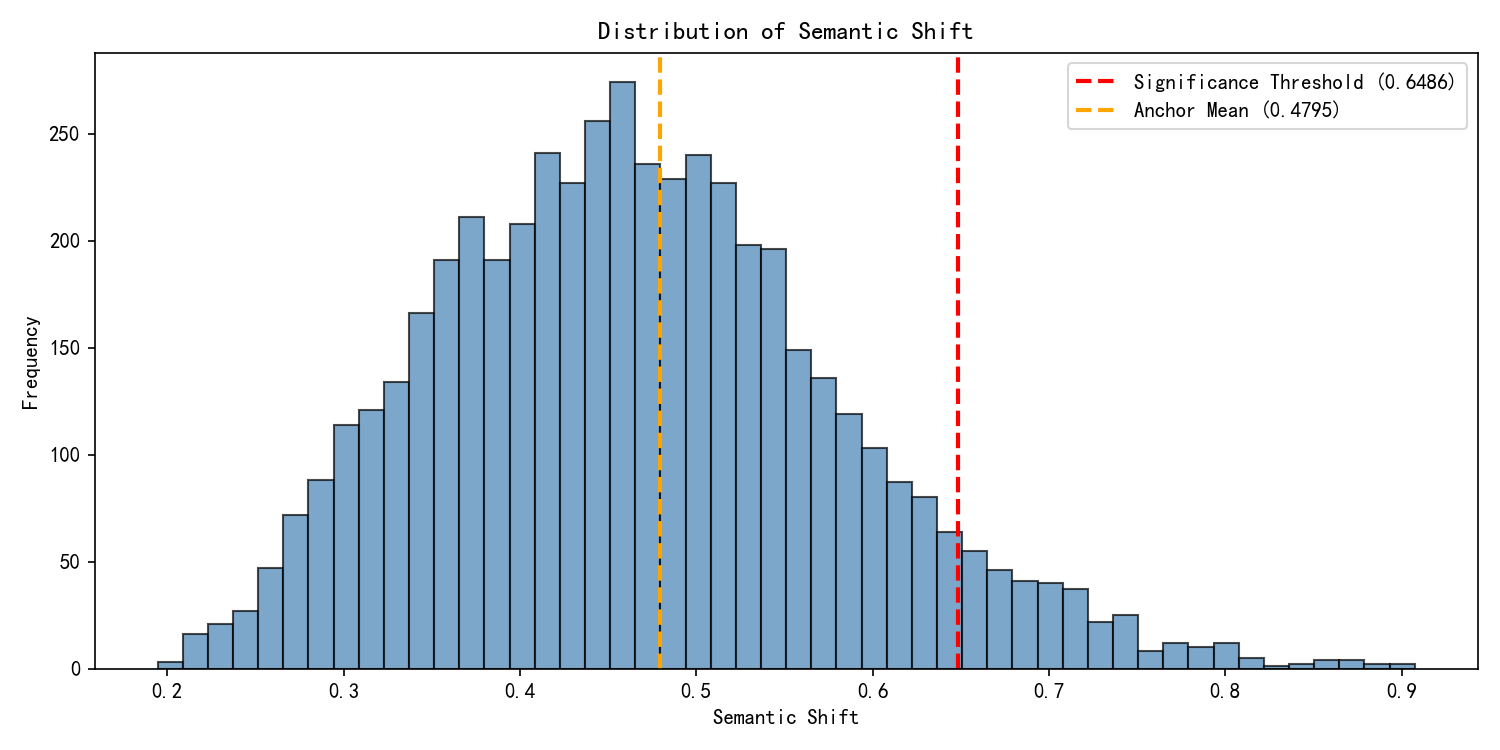
\includegraphics[width=0.88\textwidth]{shift_distribution.png}}{%
    \fbox{\parbox[c][0.18\textheight][c]{\linewidth}{\centering （插图：漂移量直方图）}}}
  \caption{高频非锚点词的漂移量分布（阈值与参照均值以竖线标示）}
  \label{fig:word-shift-dist}
\end{figure}

\begin{figure}[!htbp]
  \centering
  \IfFileExists{./figures/word/shift_top20_auto.png}{%
    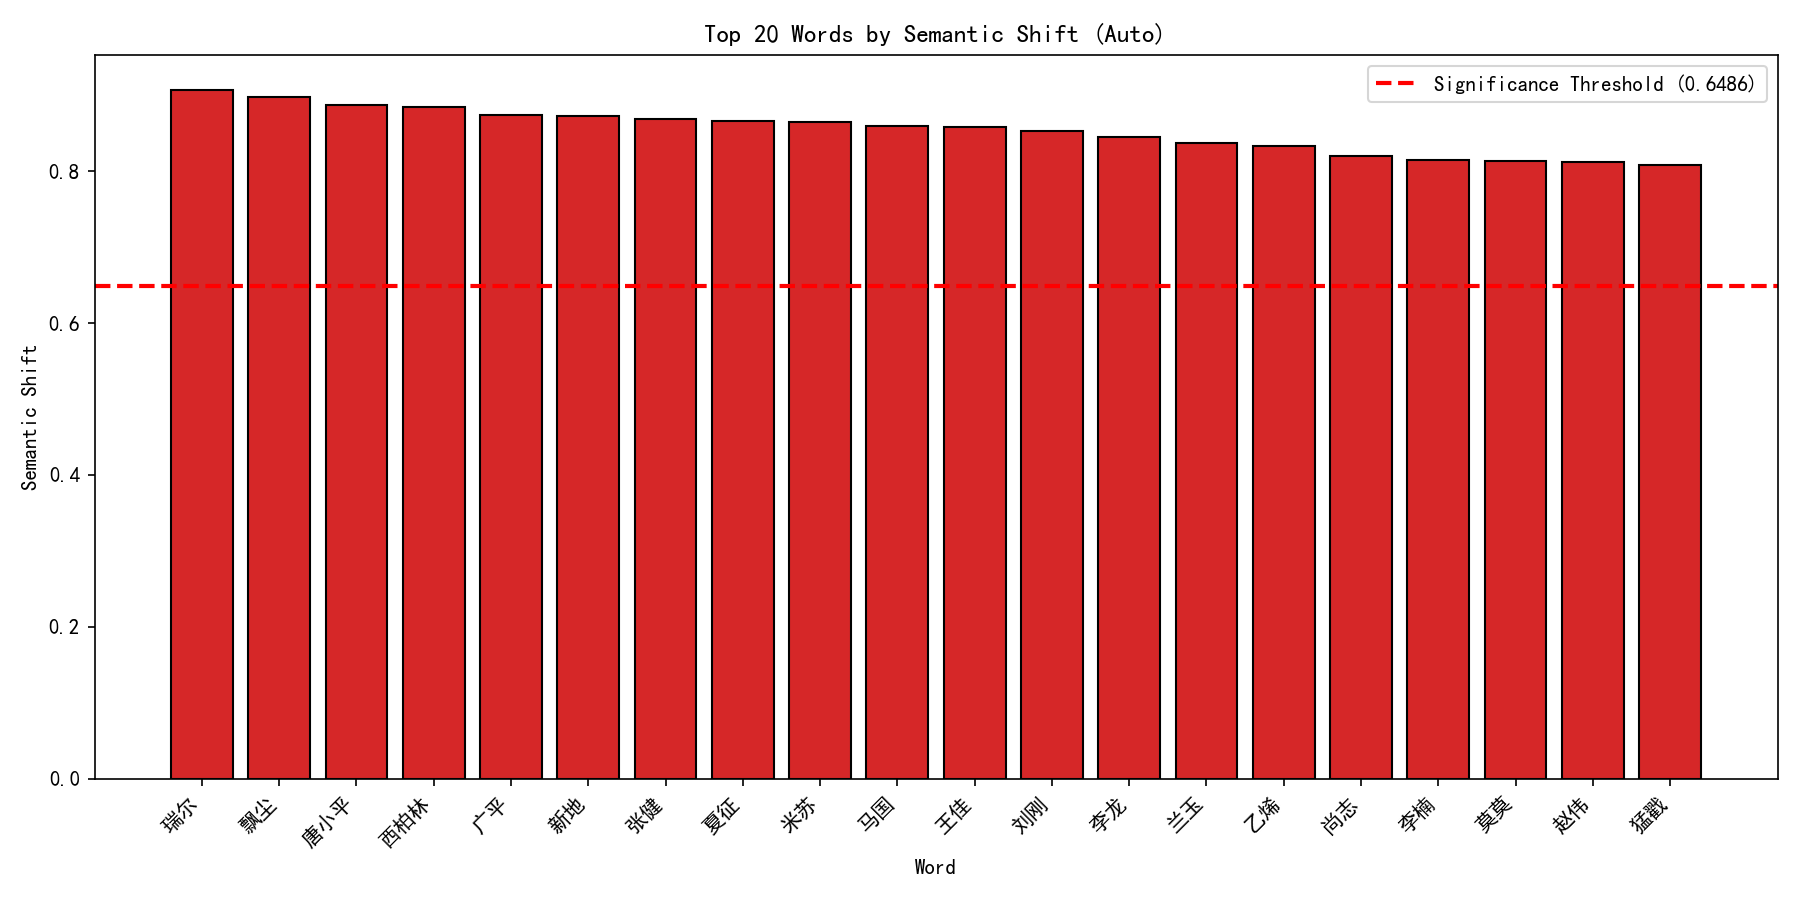
\includegraphics[width=0.88\textwidth]{shift_top20_auto.png}}{%
    \fbox{\parbox[c][0.18\textheight][c]{\linewidth}{\centering （插图：漂移量自动 Top 20）}}}
  \caption{漂移量自动 Top 20（多为低频专有名词）}
  \label{fig:word-shift-auto}
\end{figure}

\begin{figure}[!htbp]
  \centering
  \IfFileExists{./figures/word/shift_top20_selected.png}{%
    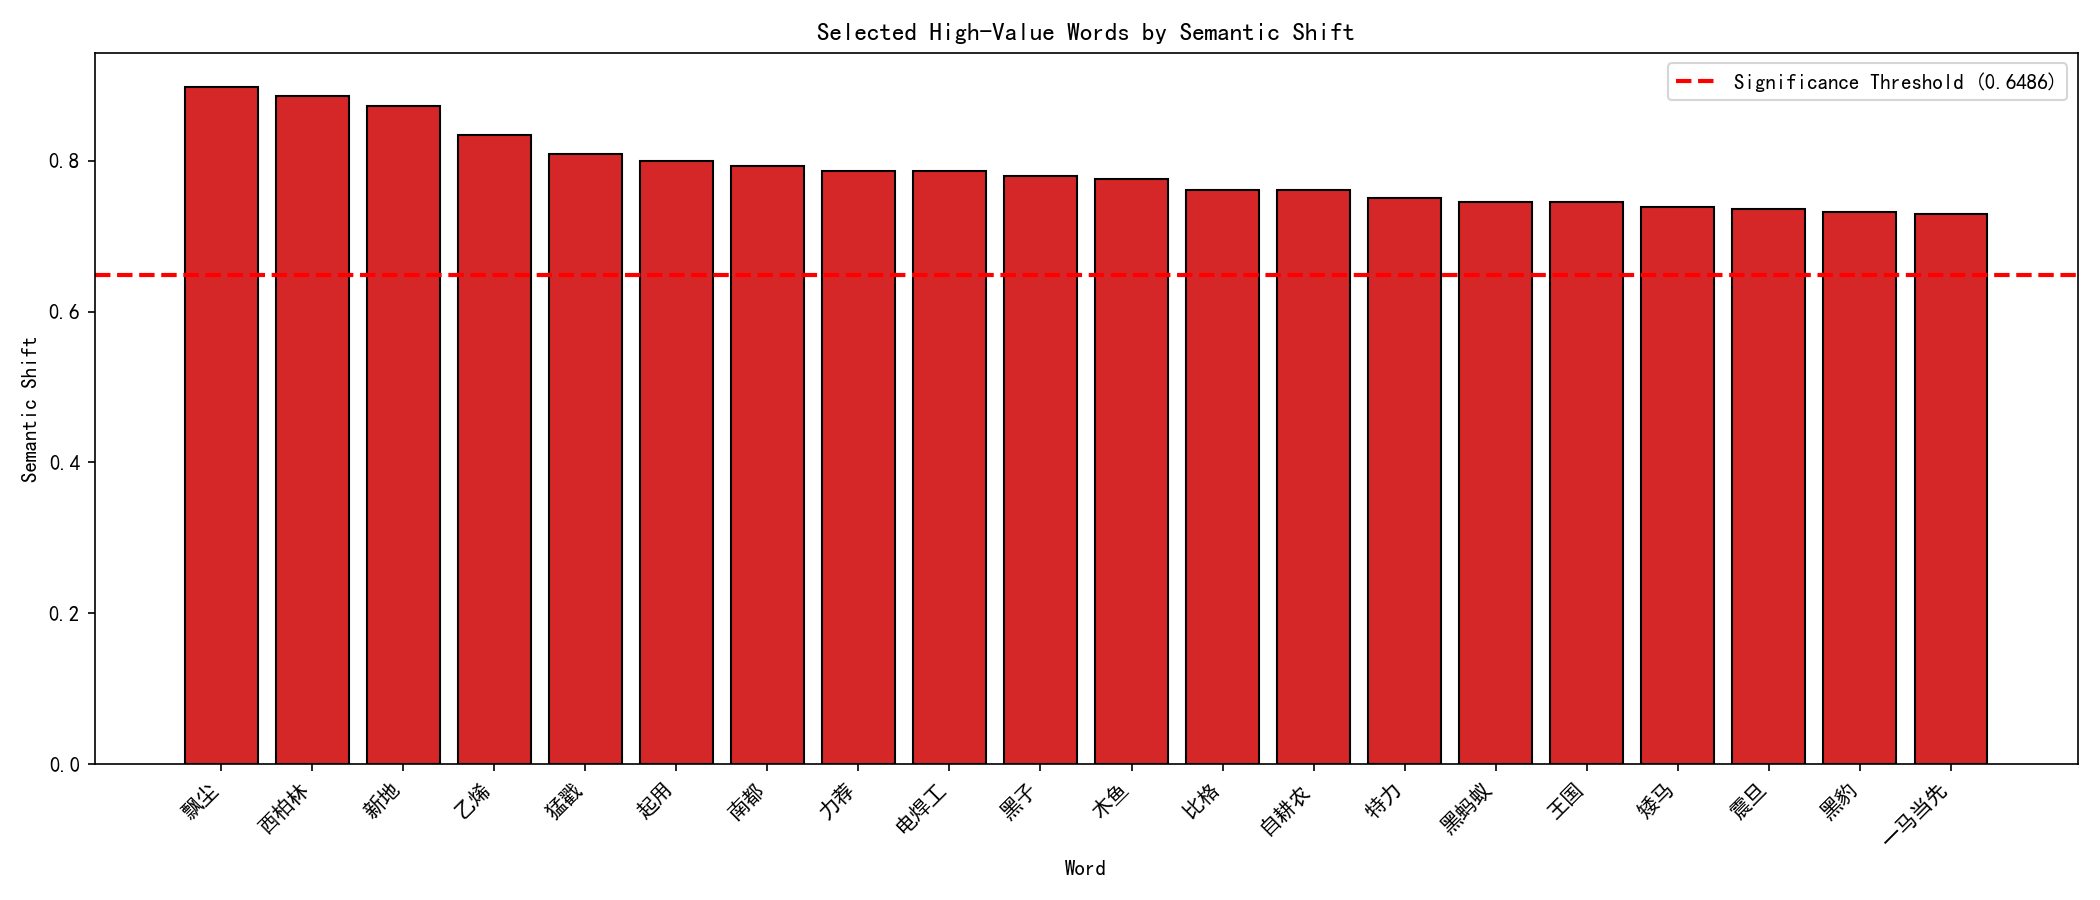
\includegraphics[width=0.92\textwidth]{shift_top20_selected.png}}{%
    \fbox{\parbox[c][0.18\textheight][c]{\linewidth}{\centering （插图：人工筛选高价值漂移词）}}}
  \caption{人工筛选的高价值漂移词}
  \label{fig:word-shift-selected}
\end{figure}

\subsection{邻域重合度（Jaccard）}

\subsubsection{定义与公式}
除方向外，可比较邻域结构。对词 $w$，在人民日报空间与对齐后微博空间中分别取其 $k$ 近邻集合
 $N_{\mathrm{rm}}(w)$、$N_{\mathrm{wb}}(w)$（在各自词表与余弦度量下），定义
\begin{equation}
  J_k(w)
  = \frac{\lvert N_{\mathrm{rm}}(w)\cap N_{\mathrm{wb}}(w)\rvert}{\lvert N_{\mathrm{rm}}(w)\cup N_{\mathrm{wb}}(w)\rvert}
\end{equation}

\subsubsection{指标含义}
$J_k(w)$ 越接近 $1$，表示两域在该词处的邻域越重合；越接近 $0$，表示邻域几乎完全重排。

\subsubsection{汇总口径与结果分析}
本文不对 $J_k(w)$ 另行构造假设检验或拒绝域，仅在 $k\in\{10,50\}$ 上报告其在考察词上的
\textbf{样本平均} $\overline{J}_k$，用作与 $\mathrm{Shift}(w)$ 并列的粗粒度对照。

当前 $\overline{J}_{10}\approx0.0904$：在“各取 $10$ 个最近邻”的\textbf{紧局部}下，
两域邻域集合的 Jaccard 重合度平均不足 $0.1$，直观上相当于每个词周围约 $10$ 个近邻里
\textbf{常不足 $1$ 个}能在另一侧的近邻表中保留--邻域几乎整体更换，说明对齐主要校正了
\textbf{全局刚体分量}，并未把每个词周围的细粒度共现结构也一并拉齐。

将邻域放宽到$k=50$ 后，$\overline{J}_{50}\approx0.1602$ 有所抬升：更大 $k$ 会把更外圈的、由高频功能词
与通用搭配支撑的近邻纳入集合，两侧偶然重合的词语增多，Jaccard 因而上升，但绝对水平仍低，
\textbf{重排仍是主导现象}。

与 $\mathrm{Shift}(w)$ 只看对齐后\textbf{单一方向}不同，$J_k(w)$ 直接比较两侧\textbf{词集合}，
对“邻域语义场是否一致”给出独立刻画。二者同向地指向：人民日报与微博在词级上不仅存在
方向差，还存在系统性的\textbf{局部结构差}。

\FloatBarrier

\section{联合 PCA-50 表示}

本节构造第六、七节共用的\textbf{联合 PCA-50 坐标} $\mathbf{Z}_{\mathrm{all}}$

\subsection{动机：降维需求与联合主成分}

对齐完成后，词向量仍处于 $d=300$ 维。若在全词表上反复执行 KMeans、样本协方差估计、全点对距离统
计或子空间上的大规模普鲁克匹配，计算与存储代价高，且谱量与图形输出在论文尺度上不易稳定呈现。
因而需要\textbf{维数截断}，将分析限制在维数可控的工作子空间中。

维数截断不能直接“各自做 PCA 再比较”。若对微博与人民日报\textbf{分别}估计主成分，
两侧得到的载荷矩阵一般\textbf{不相同}，截断后的坐标系彼此旋转关系未知，\textbf{逐坐标比较}
将失去明确的几何含义。为此，本文将两域样本
\textbf{纵向拼接}后在合并矩阵上估计\textbf{同一套}主方向，并将两侧词向量\textbf{用同一载荷}
投影到 $\mathbb{R}^{50}$；这样得到的 $\mathbf{z}$ 位于\textbf{共享主子空间}内，
第六节的簇统计与第七节的几何量才可在\textbf{同一基}下解读。

上述 $\mathbf{Z}_{\mathrm{all}}$ 仅为\textbf{分析用}工作坐标，并不宣称穷尽语义信息。

\subsection{构造流程}

\subsubsection{输入与记号}
记对齐后微博、人民日报词向量矩阵分别为 $V_{\mathrm{wb}}\in\mathbb{R}^{n_{\mathrm{wb}}\times d}$、$V_{\mathrm{rm}}\in\mathbb{R}^{n_{\mathrm{rm}}\times d}$。

\subsubsection{拼接}
先对两矩阵分别做 L2 行归一化，再纵向拼接，
\begin{equation}
  V_{\mathrm{all}} = \begin{bmatrix} V_{\mathrm{wb}} \\ V_{\mathrm{rm}} \end{bmatrix}\in\mathbb{R}^{(n_{\mathrm{wb}}+n_{\mathrm{rm}})\times d}
\end{equation}
随后在 $V_{\mathrm{all}}$ 上进行主成分分析，保留 $50$ 个主成分，采用截断随机奇异值分解求解，
随机种子固定为 $42$，并将各行映射为 $\mathbf{Z}_{\mathrm{all}}$。

\subsubsection{规模与数值一致性}
当前词向量规模对应 $n_{\mathrm{wb}}=195\,202$、$n_{\mathrm{rm}}=355\,987$、$N=551\,189$。
对拼接矩阵整体投影与对分块分别投影再按行拼接，在本文数值设定下最大绝对误差在 $10^{-5}$ 量级，
故分域切片与联合矩阵在数值上可互换使用。

\begin{table}[!htbp]
  \centering
  \caption{联合 PCA 流水线关键超参数与规模}
  \label{tab:pca-pipeline}
  \begin{tabular}{@{}ll@{}}
    \toprule
    项目 & 取值 \\
    \midrule
    词数 $n_{\mathrm{wb}},\,n_{\mathrm{rm}}$ & $195\,202$ / $355\,987$ \\
    拼接行数 $N$ & $551\,189$ \\
    输出维数 & $50$ \\
    求解方式 & 截断随机 SVD \\
    随机种子 & $42$ \\
    \bottomrule
  \end{tabular}
\end{table}

\subsection{前两个主成分上的全局投影示意}

图~\ref{fig:pca-global-source-2d} 在联合 PCA 坐标的前两个主成分（$\mathrm{PC}_1$--$\mathrm{PC}_2$）平面上，对微博与人民日报各随机抽取 $8000$ 条做二维散点投影（与绘图脚本一致）。两域点云在整体上高度重叠，表明在\textbf{共享主成分体系}下，两源的全局分布可在同一低维画面内并列检视；该图仅作\textbf{定性}示意，定量指标仍以 $\mathbf{Z}_{\mathrm{all}}$ 的全部 $50$ 维及下文表格为准。

\begin{figure}[!htbp]
  \centering
  \IfFileExists{./figures/cluster/source_distribution_global_2d.png}{%
    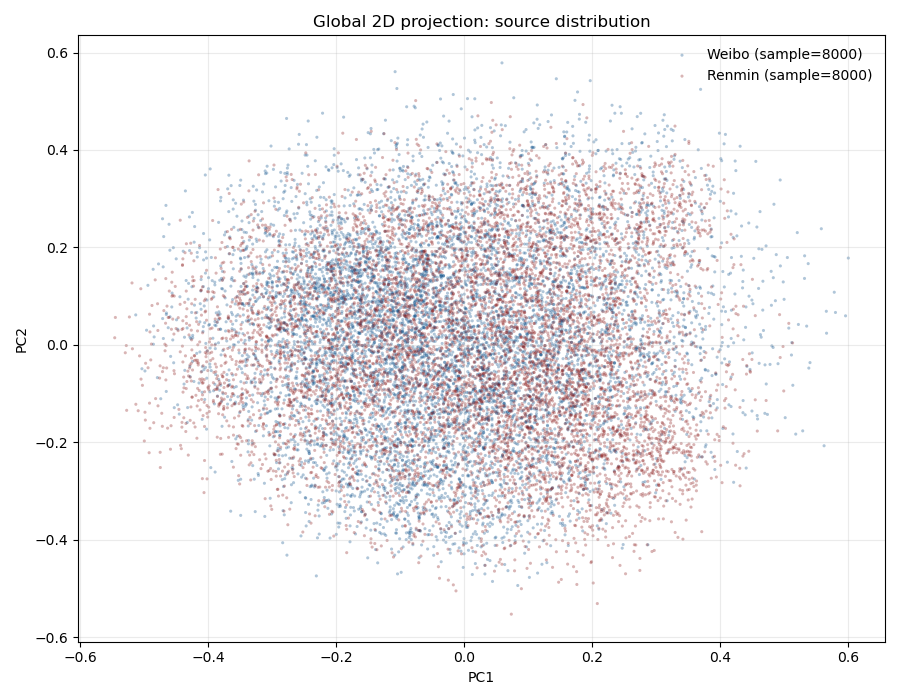
\includegraphics[width=0.8\textwidth]{source_distribution_global_2d.png}}{%
    \fbox{\parbox[c][0.22\textheight][c]{0.88\linewidth}{\centering （插图：联合 PCA 前两主成分全局投影）}}}
  \caption{联合 PCA 坐标下前两主成分的全局二维投影（随机子样本）。}
  \label{fig:pca-global-source-2d}
\end{figure}

\FloatBarrier
\section{群体级语义漂移分析}

\subsection{分析目标}
本节先在联合 PCA-50 坐标 $\mathbf{Z}_{\mathrm{all}}$ 上对两域样本一并拟合 KMeans，
得到与各词行一一对应的\textbf{合并}聚类标签，从而将词表组织为若干可比较的\textbf{群体级}语义块。
再在同一标签下，用\textbf{两组并列指标}刻画\textbf{群体级语义漂移}：\textbf{簇内组}（跨域质心漂移
与各域簇内紧致度）回答“同一合并簇内，两域点云是否同位、是否同宽”；\textbf{簇间组}（分域簇间质心
距离矩阵与轮廓系数）回答“在各域内部，簇与簇之间是否拉开、单点归属是否清晰”。

\subsection{\texorpdfstring{聚类数目 $K$ 与 KMeans 设定}{聚类数目 K 与 KMeans 设定}}

\subsubsection{\texorpdfstring{子样本上的 $K$ 诊断}{子样本上的 K 诊断}}
\label{kdiag:subsample}
簇数需在\textbf{全量}聚类之前单独论证。为控制算力，先在 $\mathbf{Z}_{\mathrm{all}}$ 
上随机抽取 $n_{\mathrm{dia}}=5\times 10^4$ 行作为\textbf{联合簇数诊断子样本}（固定随机种子，与下文诊断图绘制脚本一致），
不同候选 $K$ 上重复初始化并记录簇内平方和（惯性）及多种外部指标；据此确定主线 $K$ 后，
再在\textbf{全词表} $N\approx 5.5\times 10^5$ 行上单独拟合一次 KMeans，
下文群体级表图均基于该全量标签。

\subsubsection{手肘法：未见明确肘点}
图~\ref{fig:k-elbow} 给出子样本上惯性随 $K$（$2$--$80$）的变化。曲线在中小 $K$ 区间下降后转为\textbf{近似光滑、缓慢递减}，缺乏手肘法中常见的\textbf{斜率突变式转折点}，因而\textbf{不能}仅凭惯性--$K$ 曲线唯一敲定簇数。

\begin{figure}[!htbp]
  \centering
  \IfFileExists{./figures/cluster/elbow_method_for_optimalk.png}{%
    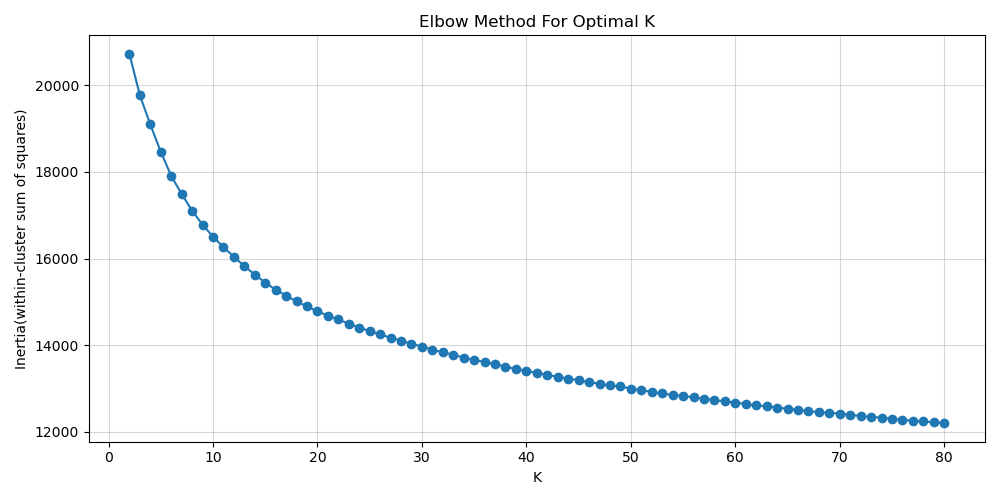
\includegraphics[width=0.88\textwidth]{elbow_method_for_optimalk.png}}{%
    \fbox{\parbox[c][0.2\textheight][c]{0.88\linewidth}{\centering （插图：手肘法惯性--$K$ 曲线）}}}
  \caption{子样本上 KMeans 惯性随簇数 $K$ 的变化：曲线整体光滑，无明显肘点。}
  \label{fig:k-elbow}
\end{figure}

\subsubsection{\texorpdfstring{多指标综合与取 $K=20$}{多指标综合与取 K=20}}
在 $K=2$--$30$ 上同步绘制惯性、轮廓系数、Calinski--Harabasz 与 Davies--Bouldin，
见图~\ref{fig:k-multi-methods}。惯性仍整体单调下降；Calinski--Harabasz 亦未呈现可分单峰。
\textbf{轮廓系数}在 $K\approx 19$--$20$ 附近达到较高水平；\textbf{Davies--Bouldin}
在 $K\approx 18$--$22$ 落入较低区间。结合多指标的一致提示与后续簇级解释的可读性，本文\textbf{取 $K=20$} 
作为群体级分析的主线簇数。

\begin{figure}[!htbp]
  \centering
  \IfFileExists{./figures/cluster/multi_methods_for_optimalk.png}{%
    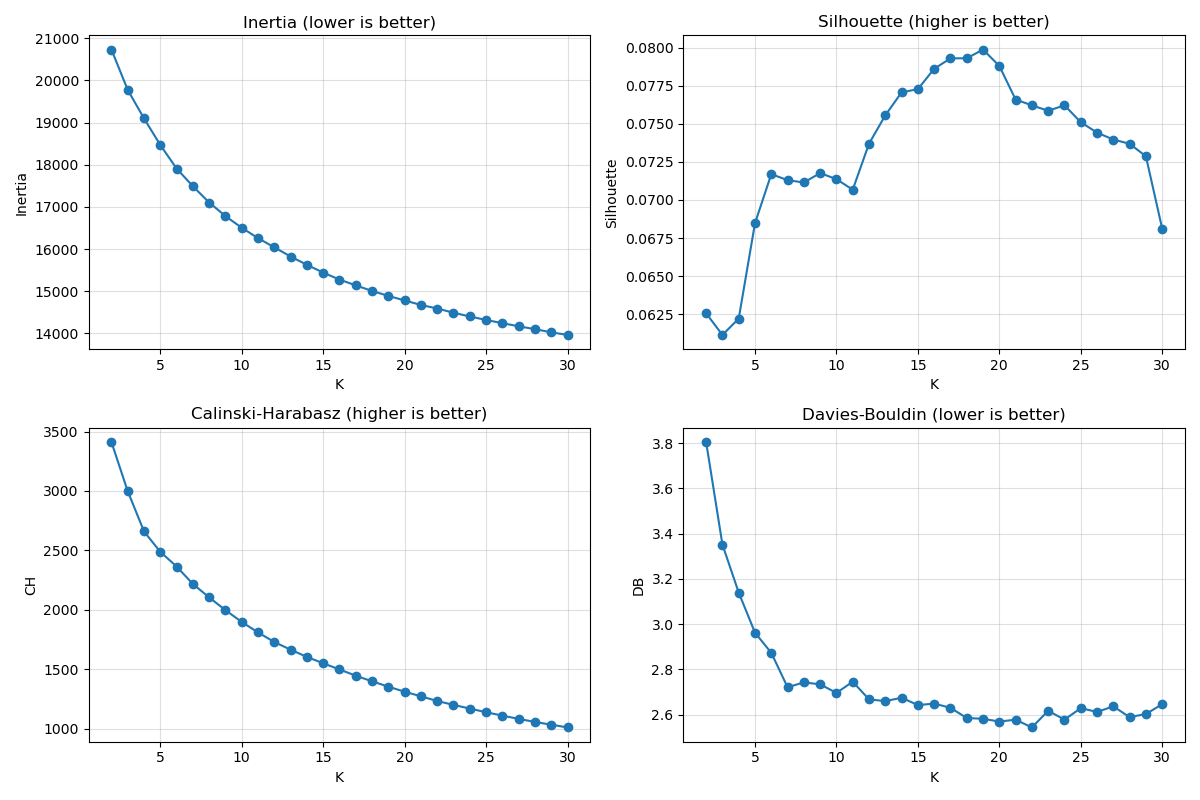
\includegraphics[width=\textwidth]{multi_methods_for_optimalk.png}}{%
    \fbox{\parbox[c][0.25\textheight][c]{\linewidth}{\centering （插图：$K=2$--$30$ 多指标联合诊断）}}}
  \caption{同一子样本上 $K=2$--$30$ 的多指标联合诊断。}
  \label{fig:k-multi-methods}
\end{figure}

\subsubsection{全量 KMeans 与标签}
在全量 $\mathbf{Z}_{\mathrm{all}}$ 上以 $K=20$ 拟合 KMeans：
初始化次数 $10$、最大迭代 $300$、随机种子 $42$，得到与各词行一一对应的\textbf{合并}簇标签，与 
$\mathbf{Z}_{\mathrm{all}}$ 一并用于下文各表与图。

\subsubsection{\texorpdfstring{$K=20$ 聚类结果的图像总览}{K=20 聚类结果的图像总览}}
图~\ref{fig:k20-source-dominance} 按簇给出两域词的
\textbf{绝对计数}堆叠条，便于直观看清各簇规模及单源主导程度；图~\ref{fig:k20-percluster-2d} 
在联合 PCA 的前两主成分平面上\textbf{分簇}叠画微博（蓝）与人民日报（红）子样本并标两域质心，
上分图对应簇 $0$--$9$，下分图对应簇 $10$--$19$。二者均为\textbf{定性}示意，
与表~\ref{tab:cluster-metrics}及后文质心漂移、簇内紧致度相互印证。

\begin{figure}[!htbp]
  \centering
  \IfFileExists{./figures/cluster/source_dominance_diagnostics_by_cluster.png}{%
    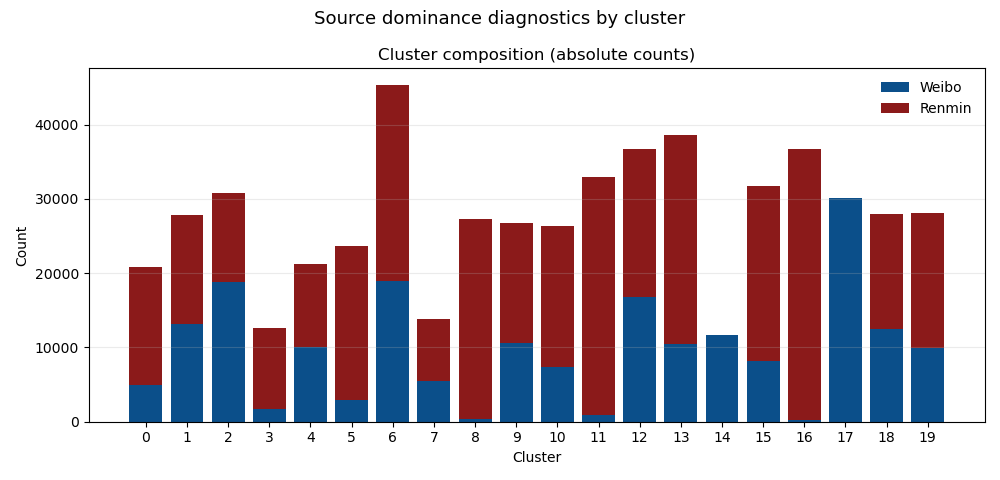
\includegraphics[width=\textwidth]{source_dominance_diagnostics_by_cluster.png}}{%
    \fbox{\parbox[c][0.2\textheight][c]{\linewidth}{\centering （插图：$K=20$ 各簇来源计数堆叠）}}}
  \caption{$K=20$ 下各簇内微博与人民日报词的绝对计数堆叠（来源占比诊断）。}
  \label{fig:k20-source-dominance}
\end{figure}

\begin{figure}[!htbp]
  \centering
  \IfFileExists{./figures/cluster/source_distribution_percluster_2d_1.png}{%
    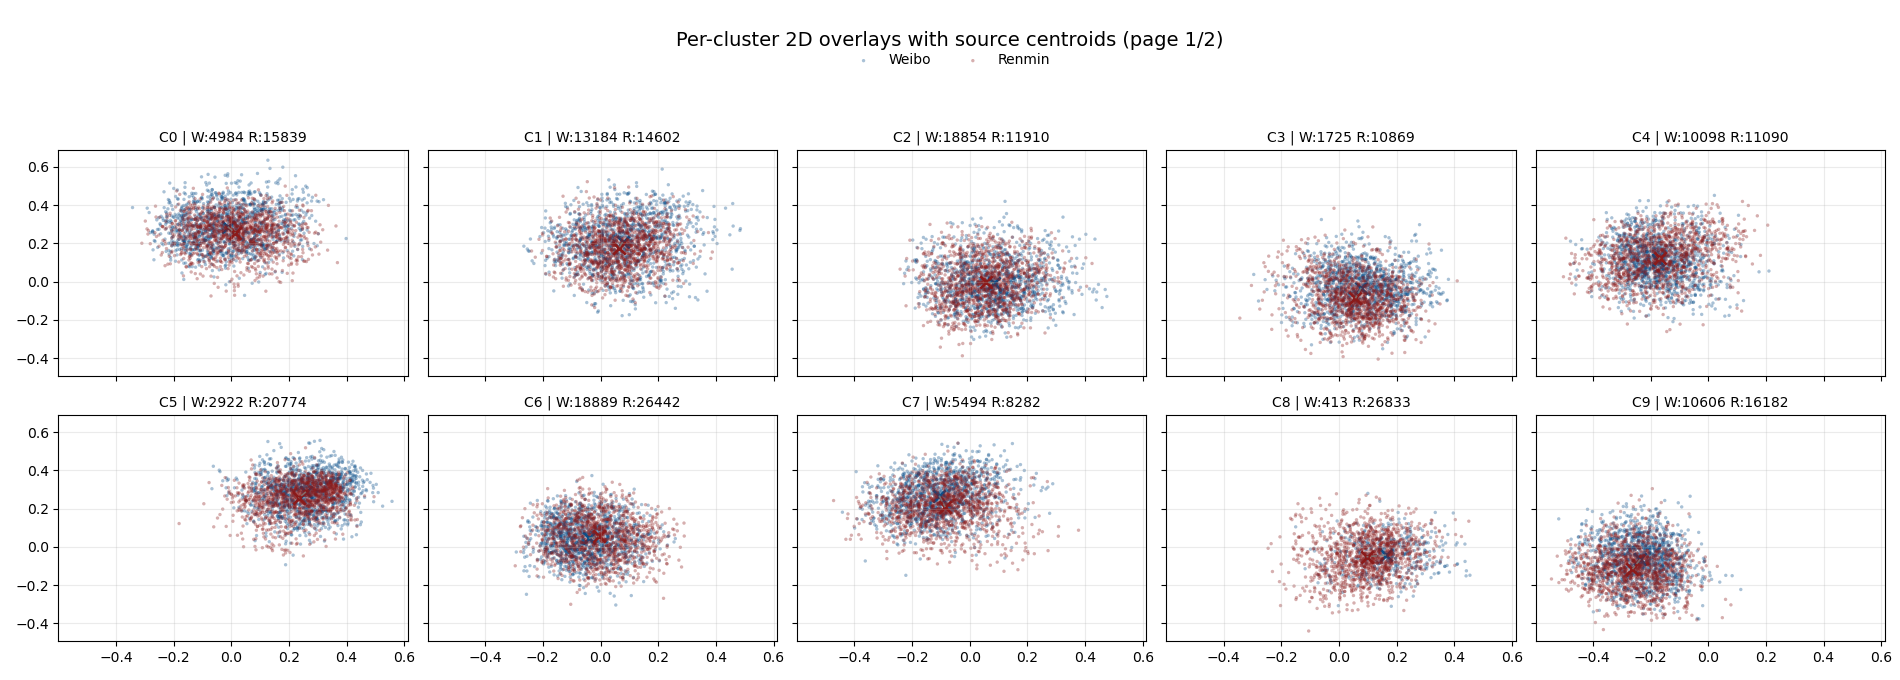
\includegraphics[width=0.92\textwidth]{source_distribution_percluster_2d_1.png}}{%
    \fbox{\parbox[c][0.18\textheight][c]{0.92\linewidth}{\centering （插图：分簇二维叠画 簇 $0$--$9$）}}}
  \\[0.6em]
  \IfFileExists{./figures/cluster/source_distribution_percluster_2d_2.png}{%
    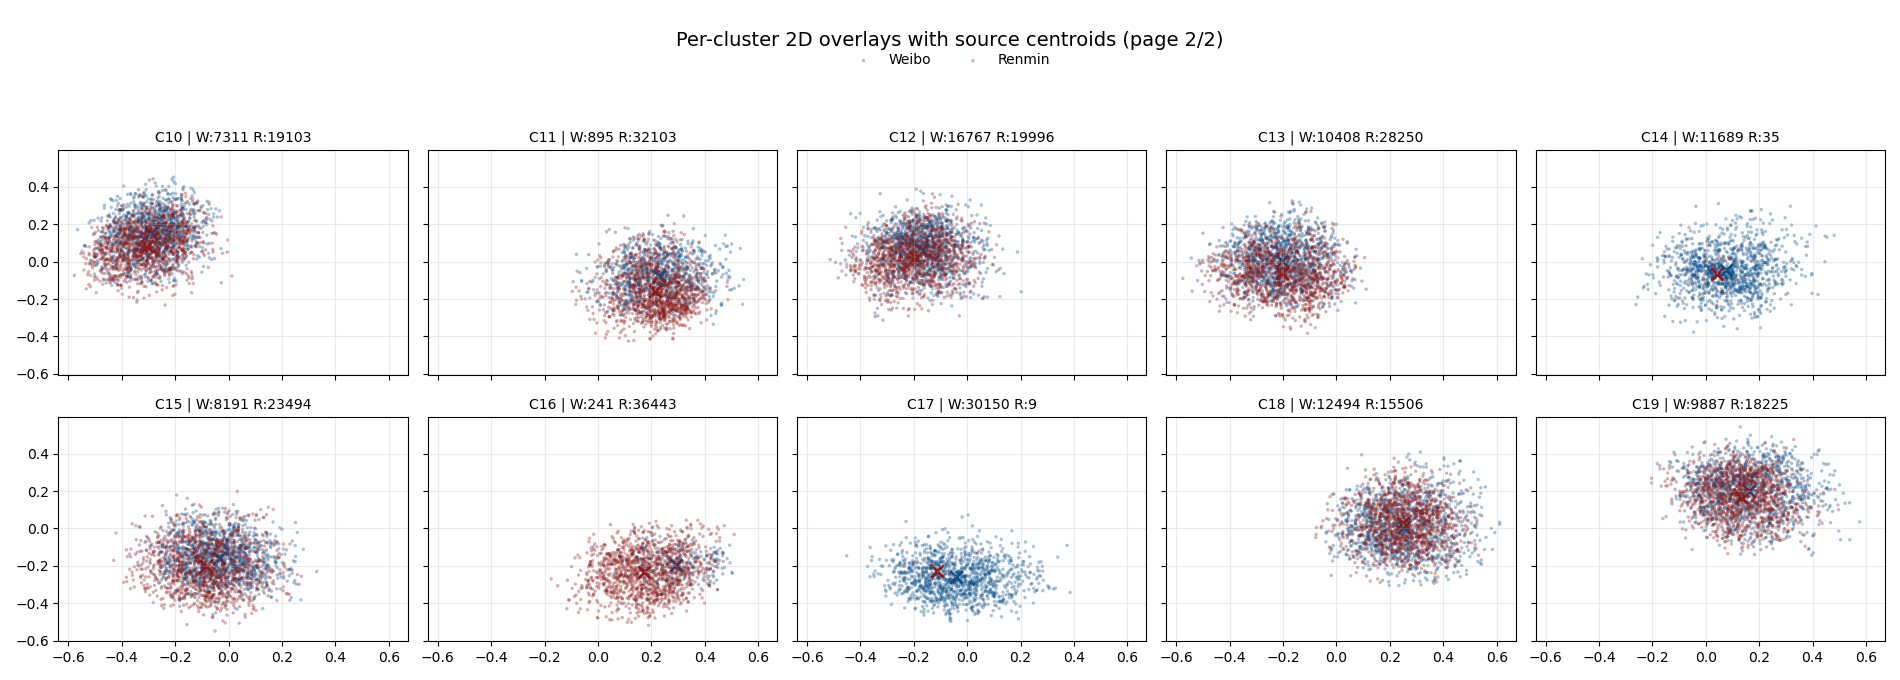
\includegraphics[width=0.92\textwidth]{source_distribution_percluster_2d_2.png}}{%
    \fbox{\parbox[c][0.18\textheight][c]{0.92\linewidth}{\centering （插图：分簇二维叠画 簇 $10$--$19$）}}}
  \caption{$K=20$ 下分簇$\mathrm{PC}_1$--$\mathrm{PC}_2$ 平面，蓝/红为两域子样本，叉号为各簇内分域质心。}
  \label{fig:k20-percluster-2d}
\end{figure}

\subsection{簇内结构：跨域质心漂移与簇内紧致度}

\subsubsection{定义与公式}
对簇 $c$，记微博、人民日报在\textbf{同一合并标签}下的索引集分别为 $\mathcal{I}^{\mathrm{wb}}_c,\mathcal{I}^{\mathrm{rm}}_c$。
先定义\textbf{跨域簇质心}（在 $\mathbf{Z}_{\mathrm{all}}$ 的行空间内对各自子块取均值）
\begin{equation}
  \boldsymbol{\mu}^{\mathrm{wb}}_c=\frac{1}{|\mathcal{I}^{\mathrm{wb}}_c|}\sum_{i\in\mathcal{I}^{\mathrm{wb}}_c}\mathbf{z}_i \qquad
  \boldsymbol{\mu}^{\mathrm{rm}}_c=\frac{1}{|\mathcal{I}^{\mathrm{rm}}_c|}\sum_{i\in\mathcal{I}^{\mathrm{rm}}_c}\mathbf{z}_i 
\end{equation}
\textbf{跨域质心漂移}取两质心的欧氏距离
\begin{equation}
  d_c = \bigl\lVert \boldsymbol{\mu}^{\mathrm{wb}}_c - \boldsymbol{\mu}^{\mathrm{rm}}_c \bigr\rVert_2
\end{equation}
再对 $s\in\{\mathrm{wb},\mathrm{rm}\}$，记 $\mathcal{I}^{(s)}_c$ 为簇 $c$ 内来源 $s$ 的索引集，定义\textbf{分域簇内质心}
\begin{equation}
  \boldsymbol{\mu}^{(s)}_c=\lvert\mathcal{I}^{(s)}_c\rvert^{-1}\sum_{i\in\mathcal{I}^{(s)}_c}\mathbf{z}_i  
\end{equation}
及\textbf{簇内均方距离}（对该域子块相对于自身簇质心的离散程度）
\begin{equation}
  C_c^{(s)} = \frac{1}{|\mathcal{I}^{(s)}_c|} \sum_{i\in\mathcal{I}^{(s)}_c}\bigl\lVert \mathbf{z}_i - \boldsymbol{\mu}^{(s)}_c \bigr\rVert_2^2 .
\end{equation}
当 $|\mathcal{I}^{\mathrm{wb}}_c|$ 或 $|\mathcal{I}^{\mathrm{rm}}_c|$ 之一为 $0$ 时，将 $d_c$ 记为缺失；本批 $K{=}20$ 下两域均非空者共 $20$ 簇。

\subsubsection{指标含义}
$d_c$ 刻画的是：在\textbf{同一个}合并簇标签下，微博块与人民日报块的\textbf{一阶位置}是否重合；
$C_c^{(s)}$ 刻画的是：在该标签下，来源 $s$ 的点云是否仍呈\textbf{薄壳或厚云}。

二者需\textbf{联合}阅读：仅有 $d_c$ 无法区分“两域整体错开”与“一侧样本极少、质心被另一侧拖拽”；
仅有 $C_c^{(s)}$ 则看不到两域整体中心是否对齐。

例如 $d_c$ 大且两侧 $C_c^{(s)}$ 均处于中等偏高区间，可解读为两域在该块上中心分离但各自仍有一定厚度；
$d_c$ 大且某一侧 $C_c^{(s)}$ 极小、对应 $|\mathcal{I}^{(s)}_c|$ 极小时，应优先怀疑\textbf{样本量驱动的质心不稳定}而非对称的跨域语义分歧。

\subsubsection{结果呈现与分析}
表~\ref{tab:cluster-metrics} 汇总各簇的 $|\mathcal{I}^{\mathrm{wb}}_c|$、$|\mathcal{I}^{\mathrm{rm}}_c|$、$d_c$、
$C_c^{\mathrm{wb}}$、$C_c^{\mathrm{rm}}$；$\{d_c\}$ 的样本均值约 $0.281$，最小值约 $0.111$（簇 $6$），最大值约 $0.454$（簇 $17$）。
图~\ref{fig:cluster-dc-panel} 与图~\ref{fig:cluster-cc-panel} 分别展示各簇的 $d_c$ 与 $C_c^{(s)}$ ，便于在同一纵轴刻度下比较簇间差异。

簇 $6$ 在 $(n_{\mathrm{wb}},n_{\mathrm{rm}})\approx(1.9,2.6)\times 10^4$ 的规模上两域样本量同阶，
$d_c$ 取全表最小，而两侧 $C_c^{(s)}$ 均在 $0.30$--$0.35$ 量级、彼此接近；这与图~\ref{fig:k20-percluster-2d} 中该簇蓝红点云
与分域质心叉号同位叠合的视觉印象一致，可视为合并标签在该块上同时覆盖两域、且两域内部松紧相仿的参照情形。

簇 $14$、$17$ 等呈现极端配比（如 $11689:35$、$30150:9$），属于单域主导簇：此时 $\boldsymbol{\mu}^{\mathrm{rm}}_c$
（或 $\boldsymbol{\mu}^{\mathrm{wb}}_c$）几乎由极少数点决定，$d_c$ 度量的是合并划分下质心的机械偏移，
不宜解释为“两域在该语义块上对称地彼此远离”。与图~\ref{fig:k20-source-dominance} 中单侧色条极薄的簇柱对照，
可快速识别此类簇并在后文可分性指标中降权解读。

此外，若干簇在 $d_c$ 中等偏高的同时，某一域 $C_c^{(s)}$ 明显低于另一域（如簇 $3$、$5$ 中人民日报侧 $C$ 显著低于微博侧），
提示同标签下两域点云的紧致性不对称：一侧更呈“低方差核”，另一侧更分散，往往与单域在簇内的话题纯度或语体集中度差异有关，
而非单纯由 $d_c$ 一个标量所能穷尽。

\paragraph{小结：} 在当前工作坐标下，簇内指标给出两点互补结果。

其一，$d_c$ 的范围跨度较大，表明不同簇的跨域中心偏移强度差异显著：既有低漂移的“共位块”（如簇 $6$），也有分域语义歧义较大的高漂移块（如簇 $14$、$17$）；
其二，$C_c^{(s)}$ 在多簇上表现出明显分域不对称，说明同一标签内两域并非仅发生“中心错位”，还伴随簇内松紧结构的系统差异。

综上，簇内结构可表述为：\textbf{不同簇的跨域质心偏移幅度不一，同簇内两域紧致度常不对称，且这种不对称程度与两域样本配比密切相关}。

\begin{figure}[htbp]
  \centering
  \IfFileExists{./figures/cluster/cluster_centroid_drift_panel.png}{%
    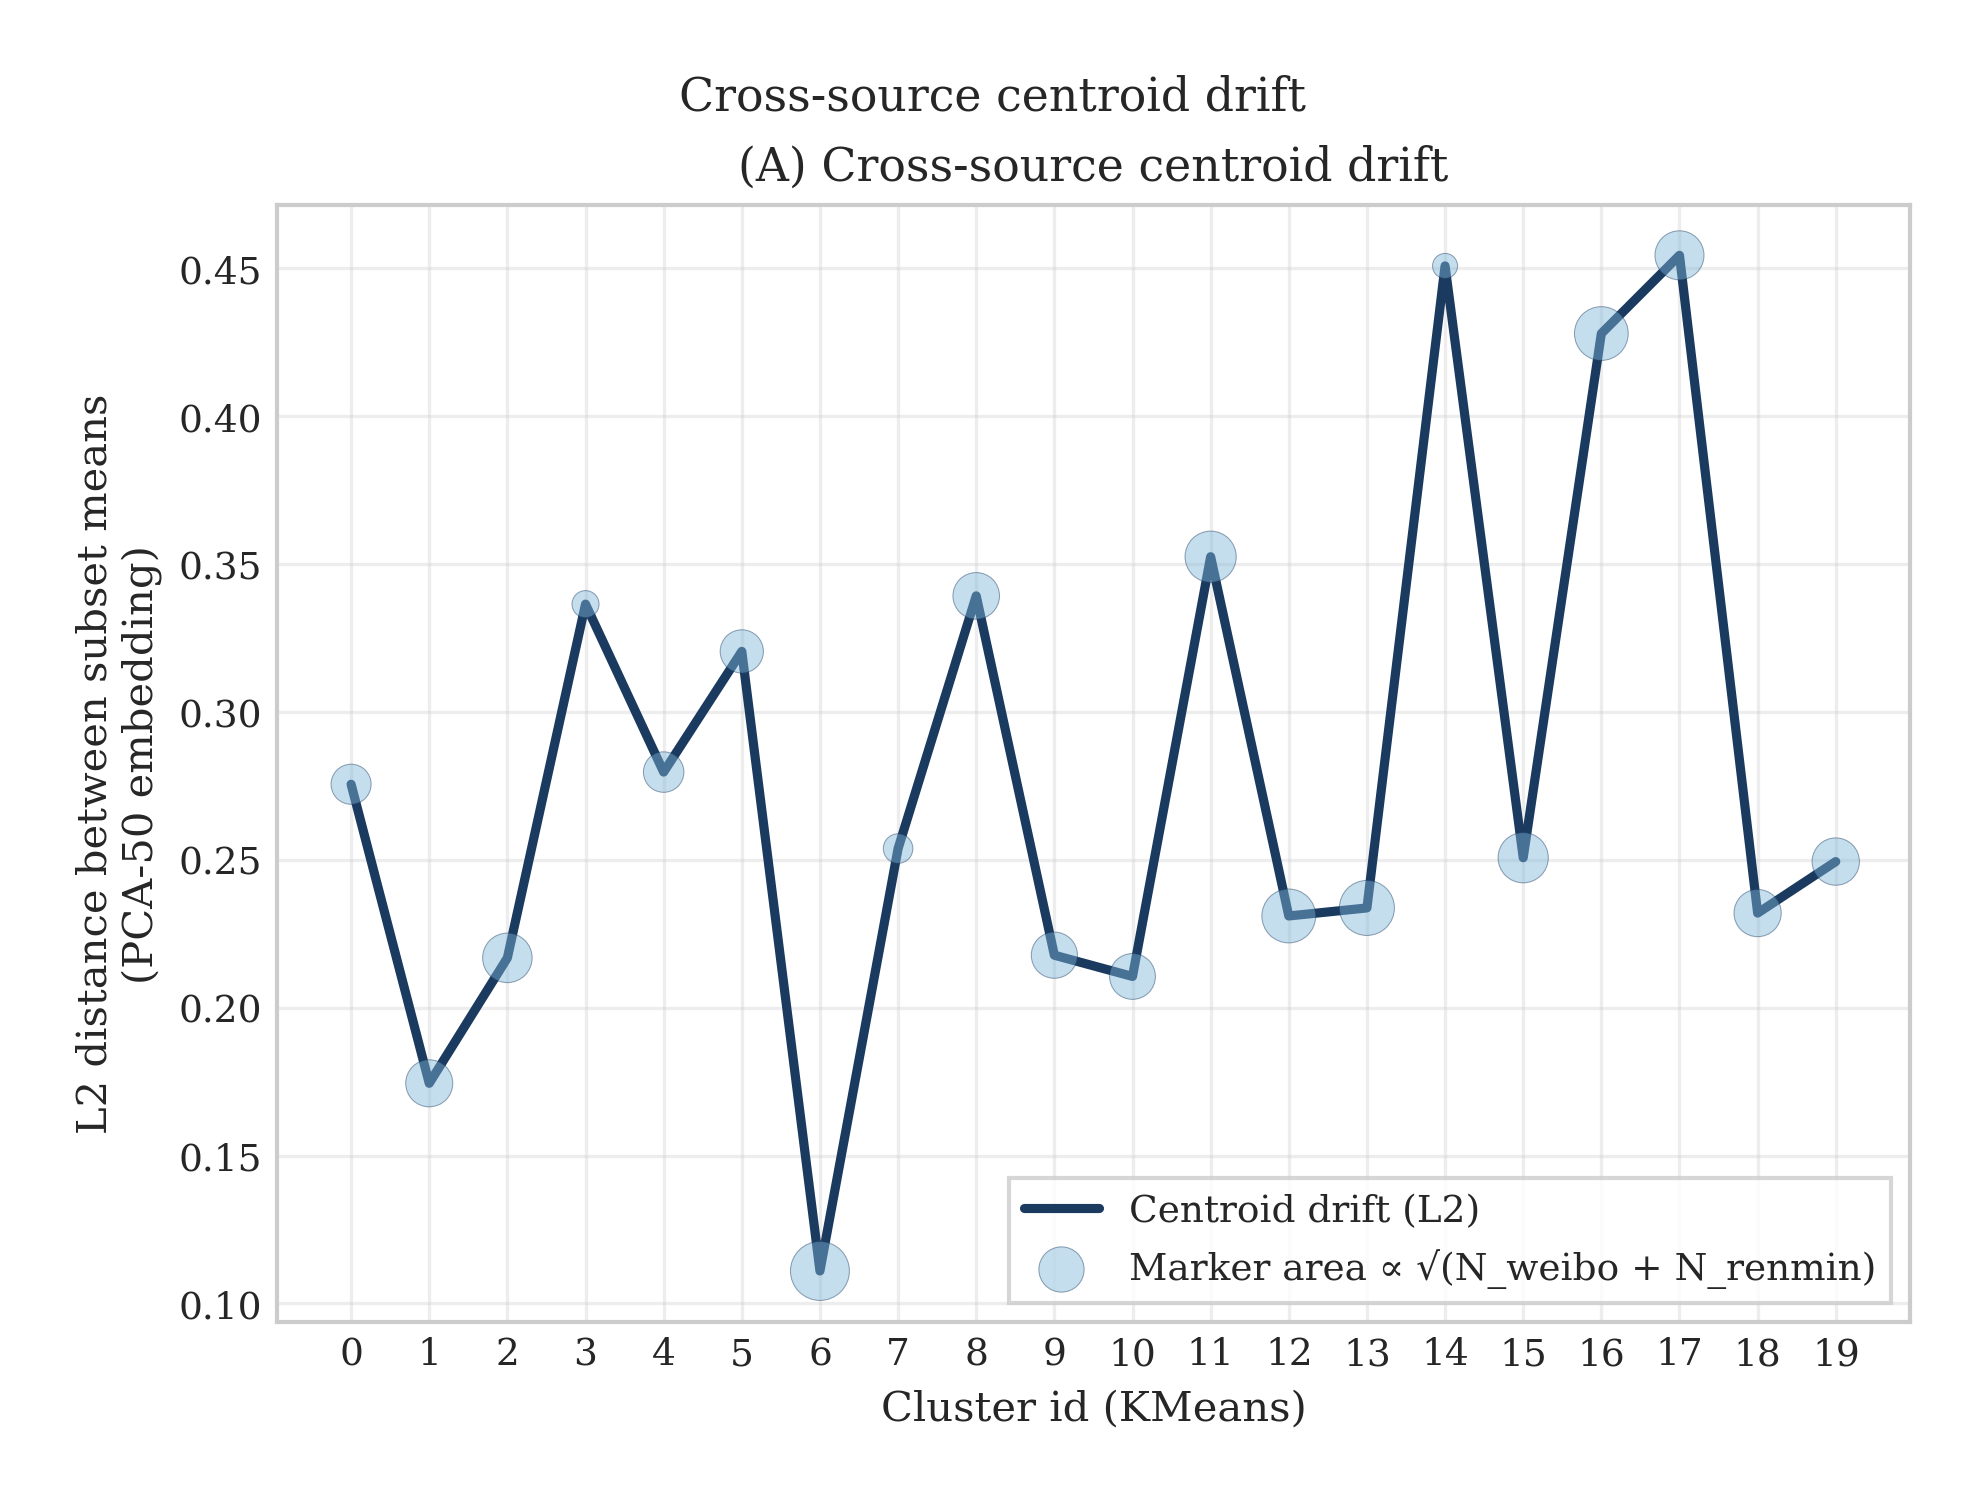
\includegraphics[width=0.88\linewidth]{cluster_centroid_drift_panel.png}}{%
    \fbox{\parbox[c][0.18\textheight][c]{0.92\linewidth}{\centering （插图：质心漂移单面板）}}}
  \caption{簇内结构：跨域质心漂移 $d_c$（与表~\ref{tab:cluster-metrics} 同源）。}
  \label{fig:cluster-dc-panel}
\end{figure}

\begin{figure}[htbp]
  \centering
  \IfFileExists{./figures/cluster/cluster_intra_compactness_panel.png}{%
    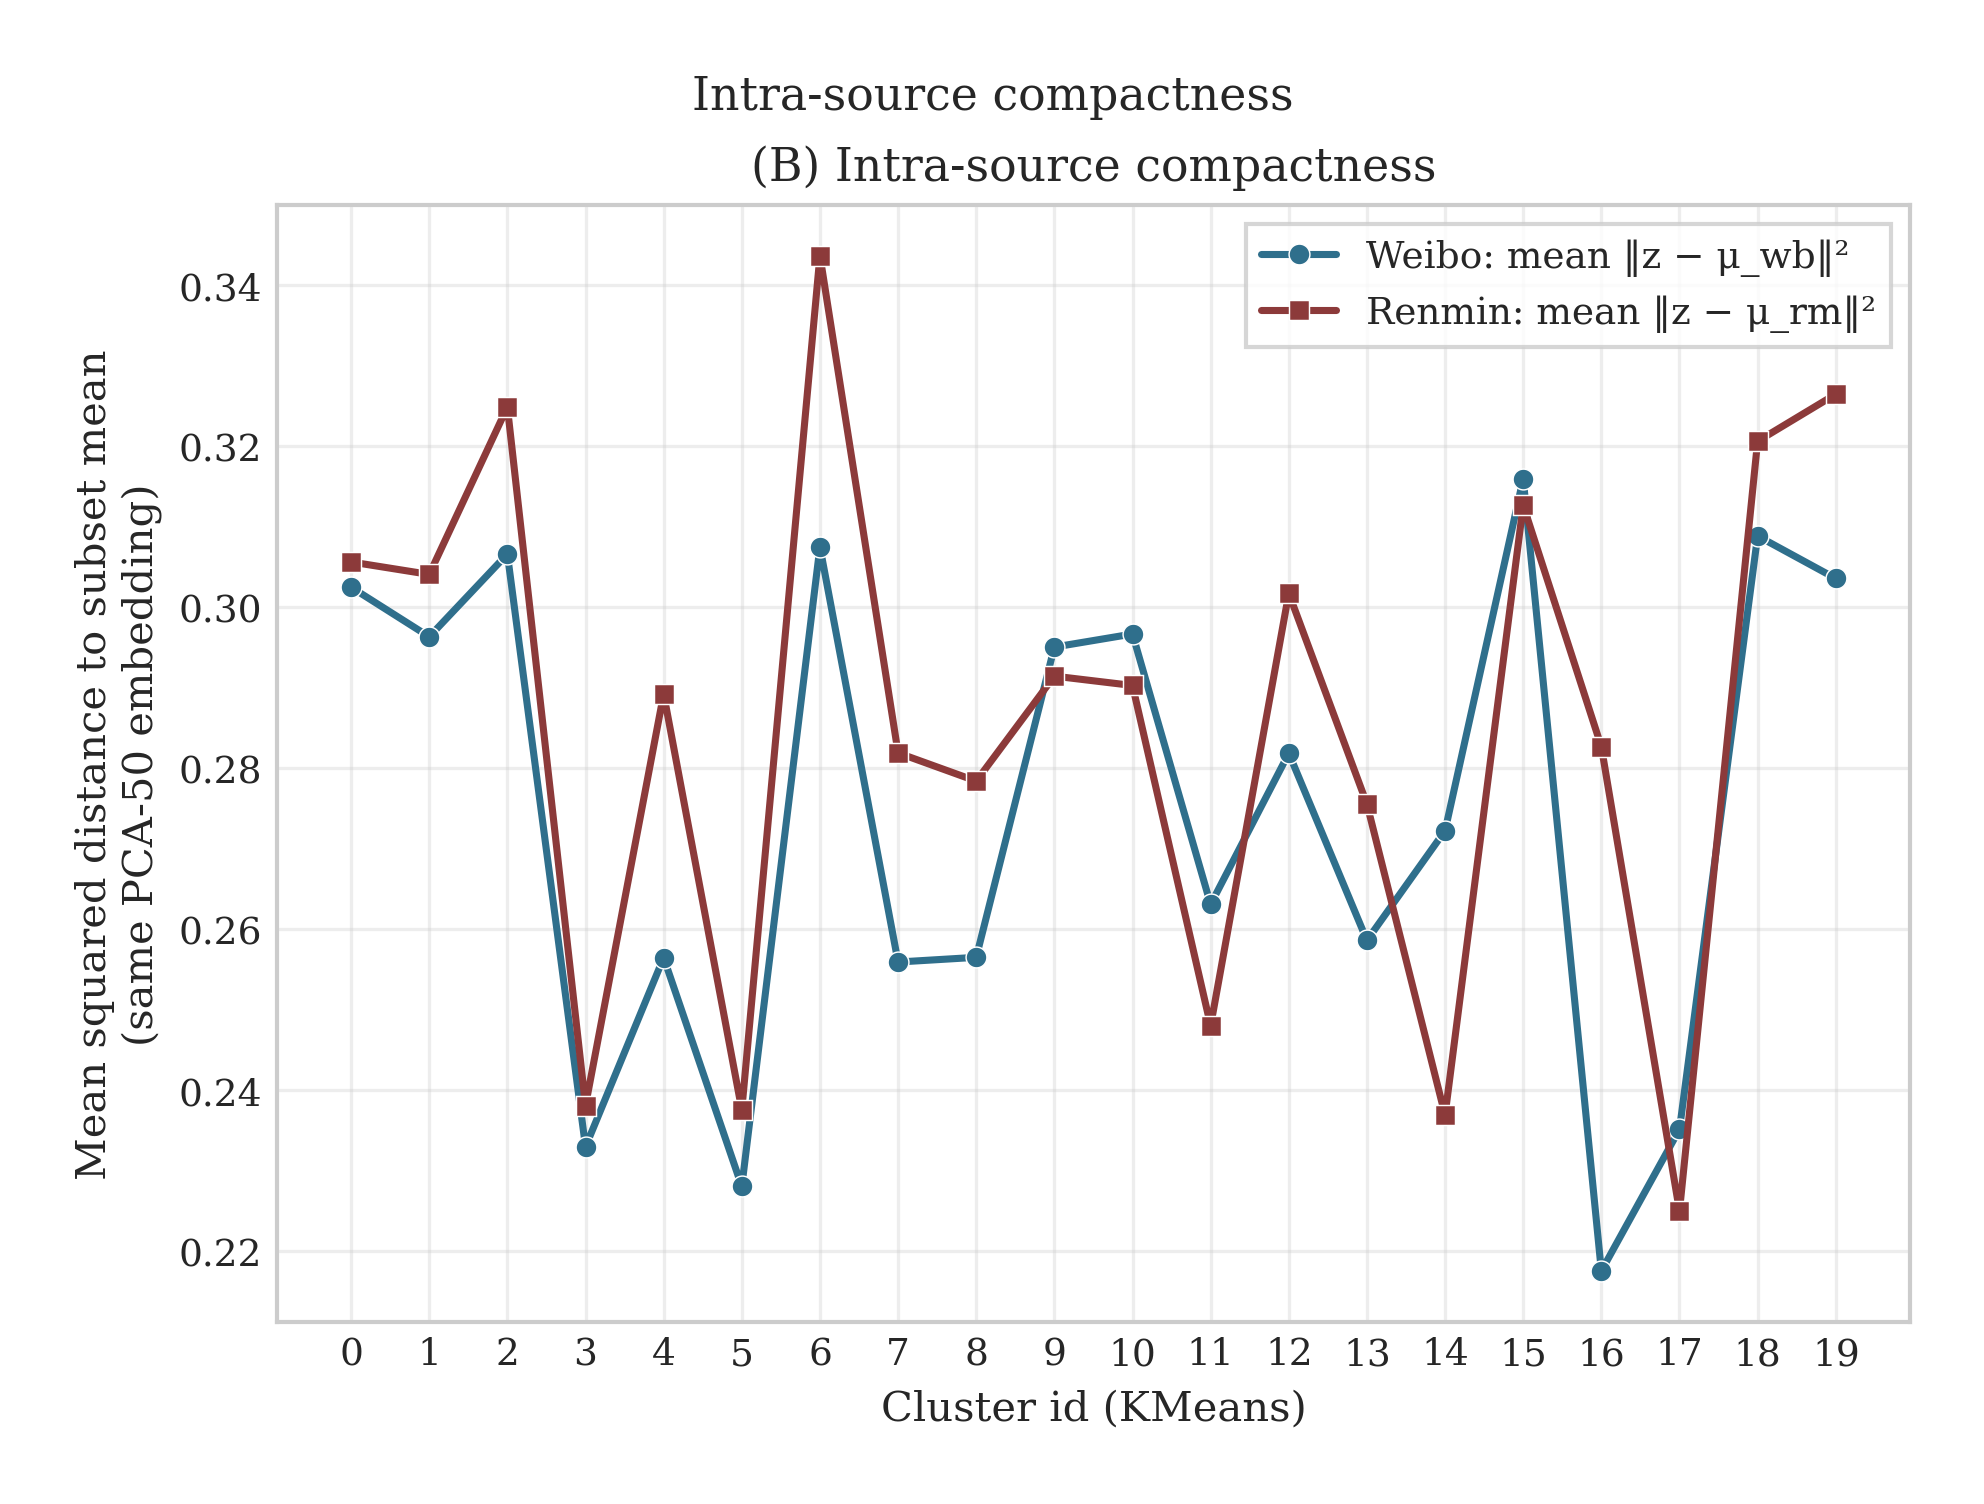
\includegraphics[width=0.88\linewidth]{cluster_intra_compactness_panel.png}}{%
    \fbox{\parbox[c][0.18\textheight][c]{0.92\linewidth}{\centering （插图：簇内紧致度单面板）}}}
  \caption{簇内结构：簇内均方距离 $C_c^{(\mathrm{wb})}$、$C_c^{(\mathrm{rm})}$（与表~\ref{tab:cluster-metrics} 同源）。}
  \label{fig:cluster-cc-panel}
\end{figure}

\begin{table}[htbp]
  \centering
  \caption{各簇样本量、跨域质心漂移与簇内紧致度（左：簇 $0$--$9$；右：簇 $10$--$19$）}
  \label{tab:cluster-metrics}
  {\tablesemismall
  \renewcommand{\arraystretch}{1.06}
  \begin{minipage}[t]{\dimexpr0.5\textwidth-0.28em\relax}
    \centering
    \begin{tabular}{@{}rrrrrr@{}}
      \toprule
      $c$ & $|\mathcal{I}^{\mathrm{wb}}_c|$ & $|\mathcal{I}^{\mathrm{rm}}_c|$ & $d_c$ & $C_c^{\mathrm{wb}}$ & $C_c^{\mathrm{rm}}$ \\
      \midrule
      0 & 4984 & 15839 & 0.2756 & 0.3025 & 0.3056 \\
      1 & 13184 & 14602 & 0.1744 & 0.2963 & 0.3041 \\
      2 & 18854 & 11910 & 0.2169 & 0.3066 & 0.3249 \\
      3 & 1725 & 10869 & 0.3365 & 0.2330 & 0.2381 \\
      4 & 10098 & 11090 & 0.2797 & 0.2565 & 0.2892 \\
      5 & 2922 & 20774 & 0.3205 & 0.2281 & 0.2376 \\
      6 & 18889 & 26442 & 0.1110 & 0.3075 & 0.3437 \\
      7 & 5494 & 8282 & 0.2538 & 0.2559 & 0.2819 \\
      8 & 413 & 26833 & 0.3393 & 0.2565 & 0.2784 \\
      9 & 10606 & 16182 & 0.2178 & 0.2950 & 0.2914 \\
      \bottomrule
    \end{tabular}
  \end{minipage}\hspace{0.55em}%
  \begin{minipage}[t]{\dimexpr0.5\textwidth-0.28em\relax}
    \centering
    \begin{tabular}{@{}rrrrrr@{}}
      \toprule
      $c$ & $|\mathcal{I}^{\mathrm{wb}}_c|$ & $|\mathcal{I}^{\mathrm{rm}}_c|$ & $d_c$ & $C_c^{\mathrm{wb}}$ & $C_c^{\mathrm{rm}}$ \\
      \midrule
      10 & 7311 & 19103 & 0.2106 & 0.2967 & 0.2903 \\
      11 & 895 & 32103 & 0.3525 & 0.2631 & 0.2480 \\
      12 & 16767 & 19996 & 0.2310 & 0.2819 & 0.3017 \\
      13 & 10408 & 28250 & 0.2337 & 0.2586 & 0.2756 \\
      14 & 11689 & 35 & 0.4509 & 0.2722 & 0.2369 \\
      15 & 8191 & 23494 & 0.2507 & 0.3159 & 0.3127 \\
      16 & 241 & 36443 & 0.4280 & 0.2176 & 0.2827 \\
      17 & 30150 & 9 & 0.4545 & 0.2351 & 0.2250 \\
      18 & 12494 & 15506 & 0.2320 & 0.3088 & 0.3206 \\
      19 & 9887 & 18225 & 0.2494 & 0.3036 & 0.3265 \\
      \bottomrule
    \end{tabular}
  \end{minipage}%
  }
\end{table}

\FloatBarrier

\subsection{簇间结构：簇间质心距离与轮廓系数}

\subsubsection{定义与公式}
在\textbf{同一组}合并标签下，已得各域簇质心族 $(\boldsymbol{\mu}^{\mathrm{wb}}_c)_{c=0}^{K-1}$、
$(\boldsymbol{\mu}^{\mathrm{rm}}_c)_{c=0}^{K-1}$。对 $s\in\{\mathrm{wb},\mathrm{rm}\}$，定义\textbf{分域簇间质心距离矩阵}
$D^{(s)}\in\mathbb{R}^{K\times K}$，其 $(c,c')$ 元为
\begin{equation}
  D^{(s)}_{c,c'} =
  \begin{cases}
    0 & c=c'\\[0.25em]
    \bigl\lVert \boldsymbol{\mu}^{(s)}_c - \boldsymbol{\mu}^{(s)}_{c'} \bigr\rVert_2 & c\neq c'
  \end{cases}
\end{equation}
其中 $\boldsymbol{\mu}^{(s)}_c$ 与簇内紧致度小节记号一致（即来源 $s$ 在簇 $c$ 内的子块均值）。

轮廓系数在各自源内的\textbf{轮廓子样本}上计算。固定上界 $n_{\mathrm{sil}}=2.5\times 10^4$；对每一来源
$s\in\{\mathrm{wb},\mathrm{rm}\}$，在全词表中属于该源的行索引里以\textbf{固定随机种子}无放回抽取至多
$n_{\mathrm{sil}}$ 行，记所得行号集合为 $\mathcal{S}_{\mathrm{sil}}^{(s)}$，则 $|\mathcal{S}_{\mathrm{sil}}^{(s)}|\leq n_{\mathrm{sil}}$。
对任意 $i\in\mathcal{S}_{\mathrm{sil}}^{(s)}$，记该行在合并划分下的簇标签为 $c(i)$，令 $a(i)$ 为 $i$ 到\textbf{同簇异点}
的欧氏距离样本均值，$b(i)$ 为 $i$ 到\textbf{最近邻簇}（按簇内点均值距离最小者）的欧氏距离样本均值，二者均在实现与上述子样本约定下计算；定义
\begin{equation}
  s(i)=\frac{b(i)-a(i)}{\max\{a(i),\,b(i)\}} 
\end{equation}
当分母为 $0$ 或邻簇不可定义时，该点轮廓按实现记为缺失或剔除；下文各源内 $s(i)$ 的均值、标准差与分位数均\textbf{仅针对}
$\mathcal{S}_{\mathrm{sil}}^{(s)}$ 上已有定义的样本点汇总。

\subsubsection{指标含义}
$D^{(\mathrm{wb})}$ 与 $D^{(\mathrm{rm})}$ 描述在某一域内部观察各簇质心时，簇与簇之间在 PCA-50 中
彼此相距多远，属于簇与簇之间的中观几何结构；与 $d_c$ 不同，$D^{(s)}$ 完全不混合两域点，
因而对“合并簇是否在分域几何上同样可分”给出并列对照。

$s(i)$ 则把问题推进到点级边界：
在固定标签与 $\mathcal{S}_{\mathrm{sil}}^{(s)}$ 上，样本点更接近自己的簇还是更接近最近的外簇；其源内均值偏低，往往意味着簇间重叠大
或标签对自然语义边界的切割偏粗。

\subsubsection{结果呈现与分析}
图~\ref{fig:separability-heatmap} 在统一色标下并排展示 $D^{(\mathrm{wb})}$ 与 $D^{(\mathrm{rm})}$。
若两侧大块亮暗格局相近，说明合并簇在分域质心几何上具有一致的疏密骨架，KMeans 划分在两域中结构同形；
若某一侧出现更细碎的高亮块或主轴方向改变，则需回到表~\ref{tab:cluster-metrics} 与图~\ref{fig:k20-source-dominance}，
核查是否由单域主导、质心受极少数点牵制等样本结构效应引起，而不宜直接解释为“该域可分性更好或更差”。

与簇内指标对照：$D^{(s)}$ 刻画簇间相对位置，$d_c$ 刻画簇内两域相对位置；二者共享同一套质心估计，但聚合层次不同。
对簇 $14$、$17$ 等极端配比簇，$D^{(s)}$ 中涉及该簇的行或列仍可能显示较大簇间距离，但其中一侧质心本身可能已由另一域缺席近似决定，
此时热力图上的高对比度更多是标签与样本支撑不匹配的副产品。

图~\ref{fig:separability-violin} 给出各源 $\mathcal{S}_{\mathrm{sil}}^{(s)}$ 上 $s(i)$ 的分布：微博侧均值约 $0.067$、人民日报侧约 $0.077$，
标准差分别约 $0.092$ 与 $0.080$。均值略为正，说明平均而言点仍略靠近本簇，但整体不高，
与“$K=20$ 的合并划分在 PCA-50 欧氏几何下边界并不锋利”的判断相容；
较大的标准差则说明 $\mathcal{S}_{\mathrm{sil}}^{(s)}$ 内 $s(i)$ 分化明显：既有轮廓清晰的点，也有贴近簇界或受最近邻簇牵拉强烈的点，
分布呈长尾或弥散形态。

\paragraph{小结：} 在当前工作坐标下，簇间指标给出两点结论。

其一，$D^{(\mathrm{wb})}$ 与 $D^{(\mathrm{rm})}$ 在统一色标下呈可对照的块状疏密结构，说明两域在簇间质心几何上共享总体骨架，同时保留局部强度差异；
其二，轮廓系数在两域均为低幅正值（微博约 $0.067$、人民日报约 $0.077$）且离散度较高（标准差约 $0.092$、$0.080$），表明多数点仍更接近本簇，但边界竞争在相当范围内存在。

综上，群体级结构可表述为：\textbf{两域簇间质心几何骨架总体可比，边界呈“弱正轮廓、较高离散”的偏软形态，且相关统计量的解释权重随簇内样本支撑强弱而变化}。

\begin{figure}[htbp]
  \centering
  \IfFileExists{./figures/cluster/cluster_separability_intercluster.png}{%
    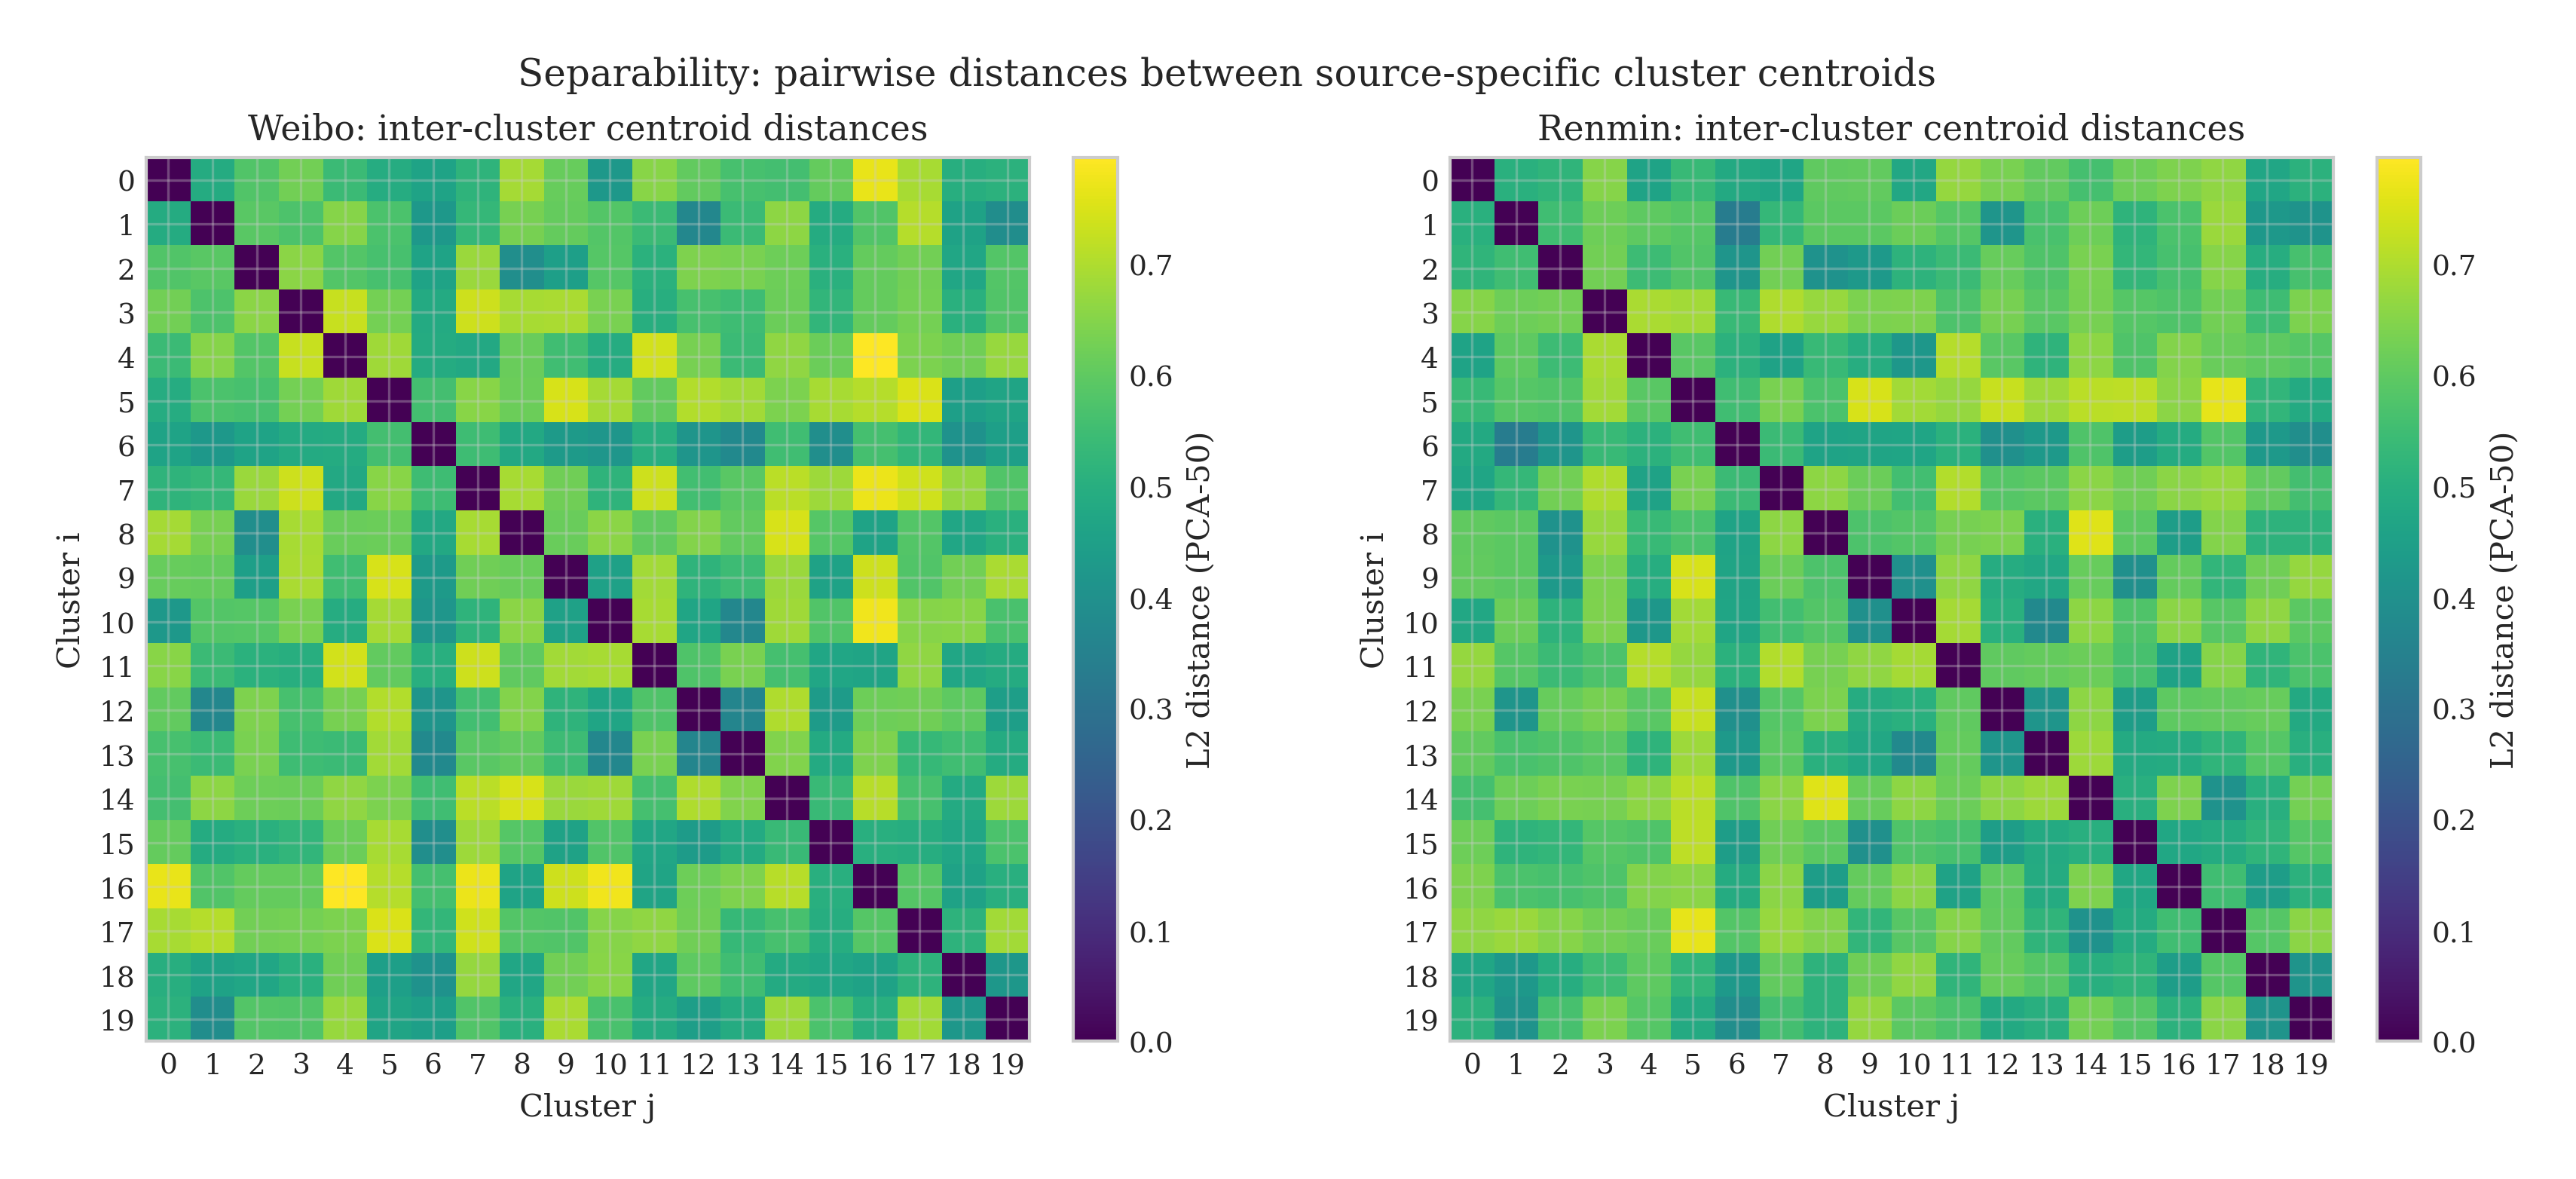
\includegraphics[width=1\textwidth]{cluster_separability_intercluster.png}}{%
    \fbox{\parbox[c][0.2\textheight][c]{\linewidth}{\centering \texttt{cluster\_separability\_intercluster.png}}}}
  \caption{可分性：微博侧（左）与人民日报侧（右）簇间质心距离热力图（同一色标）。}
  \label{fig:separability-heatmap}
\end{figure}

\begin{figure}[htbp]
  \centering
  \IfFileExists{./figures/cluster/cluster_separability_silhouette.png}{%
    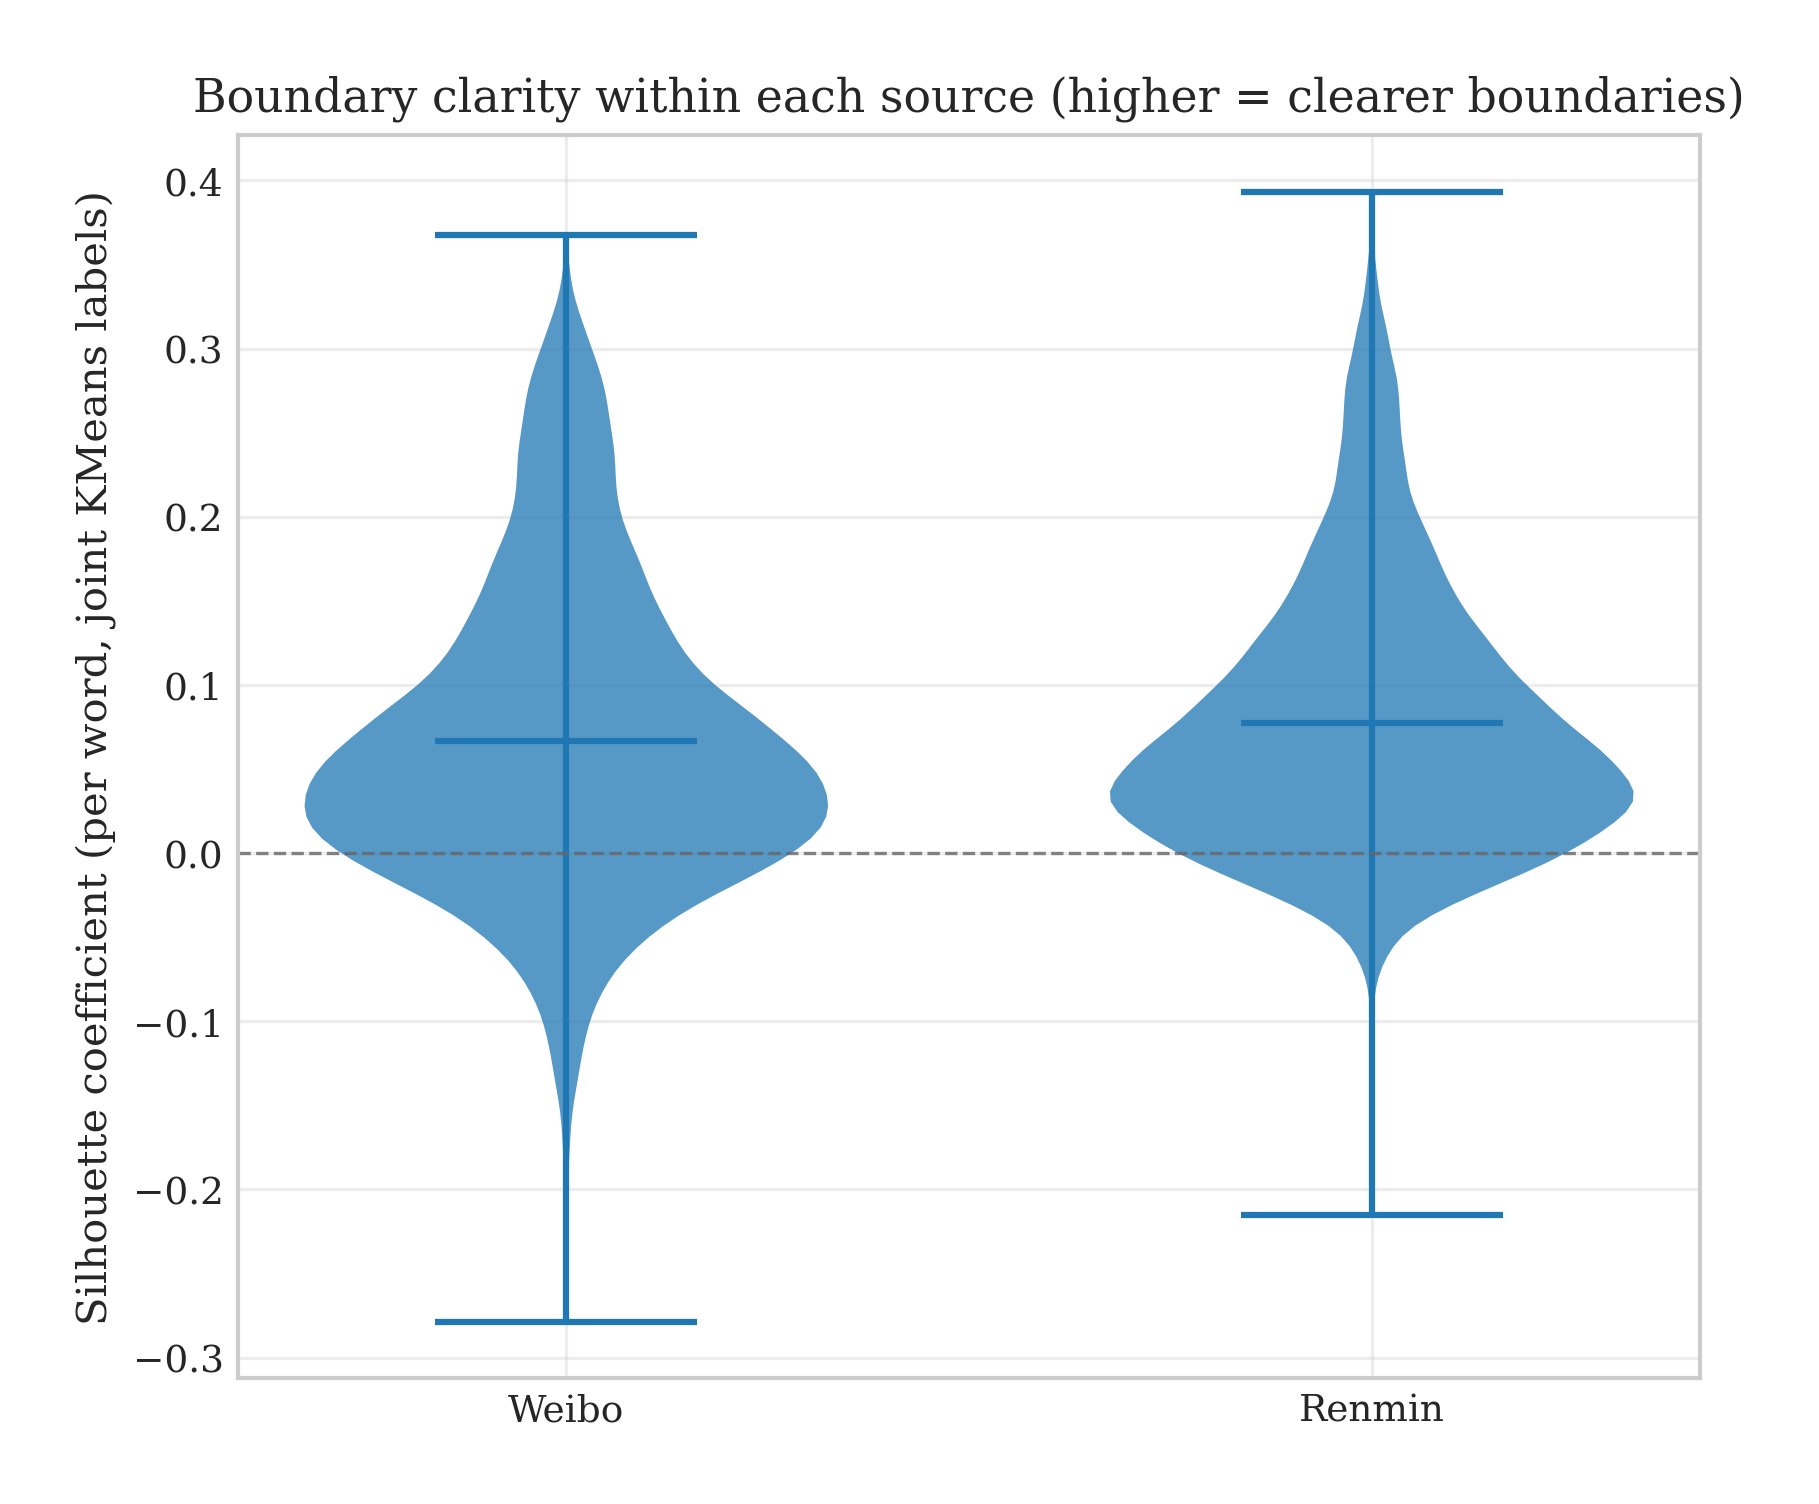
\includegraphics[width=0.88\textwidth]{cluster_separability_silhouette.png}}{%
    \fbox{\parbox[c][0.16\textheight][c]{0.62\linewidth}{\centering \texttt{cluster\_separability\_silhouette.png}}}}
  \caption{各源轮廓子样本 $\mathcal{S}_{\mathrm{sil}}^{(s)}$ 上 $s(i)$ 的分布（虚线为零参考线）。}
  \label{fig:separability-violin}
\end{figure}

\FloatBarrier
\section{几何级语义漂移分析}

\subsection{分析目标}
本节在\textbf{同一 PCA-50 工作坐标}
$\mathbf{Z}_{\mathrm{all}}$ 下，对微博块与人民日报块\textbf{分别}做整体估计。
叙述上并列三组互补问题：其一，\textbf{一阶尺度与局部距离分布}（随机子样本点对距离）回答点云是否
同尺度、典型弦长是否相近；其二，\textbf{二阶形态与总体广度}（样本协方差谱、条件数与对数广义方差）
回答能量在各主方向上的分配及“椭球状云”的扁平程度；其三，在\textbf{交集词}行对齐子矩阵上估计
\textbf{子空间正交普鲁克}残差，检验在已降维的工作空间里两域是否仍可由单一正交变换近似叠合。

\subsection{子样本点对距离分布}

\subsubsection{定义与公式}
对来源 $s\in\{\mathrm{wb},\mathrm{rm}\}$，在词表内按均匀分布独立抽取 $n{=}5000$ 条（随机种子固定），
记其在 PCA-50 中的行为 $\mathbf{z}^{(s)}_1,\ldots,\mathbf{z}^{(s)}_n$。

考虑所有无序点对
$(i,j)$（$i<j$），共 $M=\binom{n}{2}=1.24975\times 10^7$ 条，定义欧氏距离样本
\begin{equation}
  d^{(s)}_{ij}=\bigl\lVert \mathbf{z}^{(s)}_i-\mathbf{z}^{(s)}_j\bigr\rVert_2
\end{equation}
以 $60$ 个等宽 bins 将 $\{d^{(s)}_{ij}\}$ 归一化频数得到\textbf{经验密度直方图}；并报告样本均值
$\bar{d}^{(s)}=\frac{2}{n(n-1)}\sum_{i<j} d^{(s)}_{ij}$ 作为标量摘要。

\subsubsection{指标含义}
点对距离分布刻画的是：随机两词在 PCA-50 中对欧式距离的中心尺度。
它只使用\textbf{边际}距离信息，对形状细节（例如沿少数主方向拉长）不敏感，故应当与下文协方差谱\textbf{并列}
阅读。

\subsubsection{结果呈现与分析}
图~\ref{fig:geom-density} 给出两域直方图叠置后的形态。当前实现下 $\bar{d}^{(\mathrm{wb})}\approx0.917$、
$\bar{d}^{(\mathrm{rm})}\approx0.928$，相对差距不足 $2\%$，其几何含义是：两域点云在 PCA-50 中的\textbf{全局尺度}
（可理解为随机两点典型弦长或等效“半径”量级）基本一致，与图~\ref{fig:pca-global-source-2d} 中两域点云大体同尺度
的直观一致，即未出现一侧整体塌缩或整体膨胀。图中观察到两域尾部仅呈轻微差异：人民日报侧右尾相对略厚，
对应\textbf{少量极端远距词对}或\textbf{沿少数方向拉伸}效应更强；前者体现局部长尾点对整体距离分布的牵引，
后者体现各向异性增强。该读图结论与图~\ref{fig:geom-cov-spectrum} 的谱分解一致，可由后者进一步核查能量是否更集中于少数主方向。

\begin{figure}[htbp]
  \centering
  \IfFileExists{./figures/geometric/geometric_space_density_pairwise_hist.png}{%
    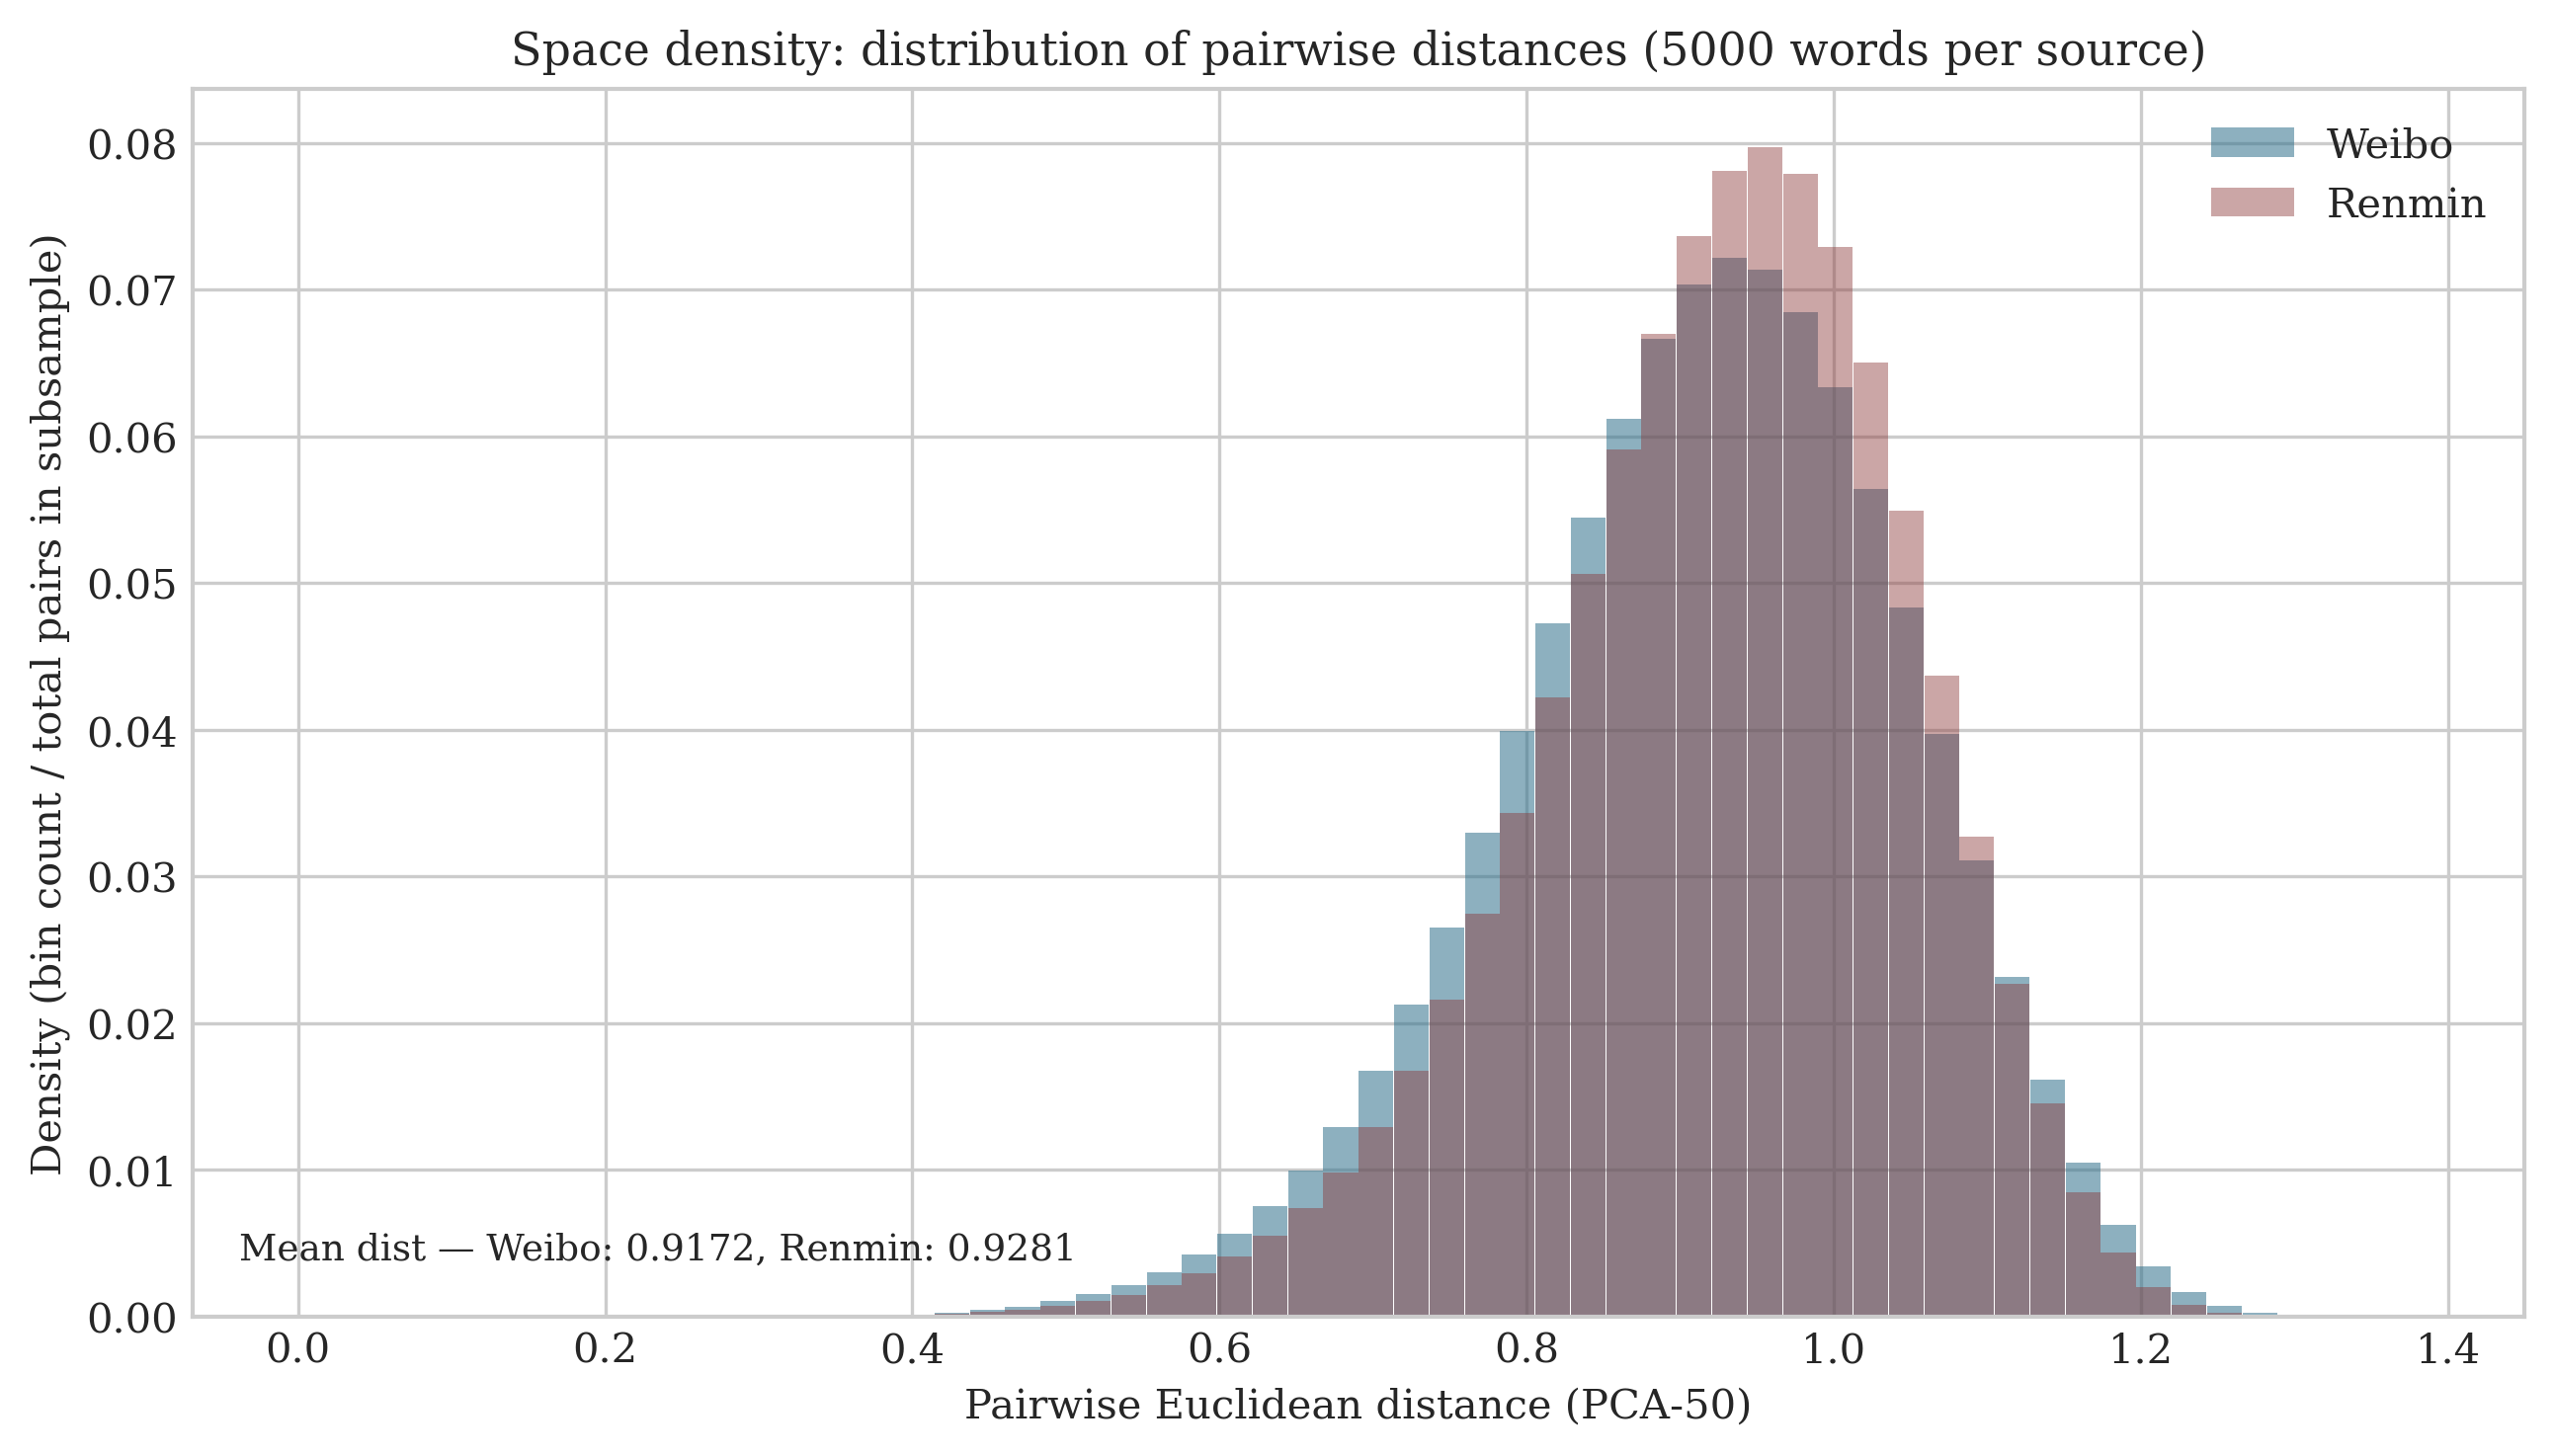
\includegraphics[width=0.88\textwidth]{geometric_space_density_pairwise_hist.png}}{%
    \fbox{\parbox[c][0.14\textheight][c]{0.88\linewidth}{\centering （插图：点对距离密度直方图）}}}
  \caption{PCA-50 空间内随机子样本的无序点对欧氏距离密度对比。}
  \label{fig:geom-density}
\end{figure}

\subsection{协方差谱与对数广义方差}

\subsubsection{定义与公式}
对来源 $s$，记其在 PCA-50 上的全体词行为中心化矩阵 $Z^{(s)}\in\mathbb{R}^{n_s\times 50}$（列已减均值），
定义样本协方差
\begin{equation}
  \hat{\boldsymbol{\Sigma}}^{(s)}=\frac{1}{n_s-1}(Z^{(s)})^{\mathsf{T}}Z^{(s)}
\end{equation}
设特征值按降序排列为 $\lambda^{(s)}_1\ge\cdots\ge\lambda^{(s)}_{50}$，则谱条件数
\begin{equation}
  \kappa^{(s)}=\lambda^{(s)}_1/\lambda^{(s)}_{50}
\end{equation}
刻画各向异性强度；对数广义方差
\begin{equation}
  \log\det\hat{\boldsymbol{\Sigma}}^{(s)}=\sum_{j=1}^{50}\log\lambda^{(s)}_j
\end{equation}
在正定情形下可视为总体离散度的一种标量概括。

\subsubsection{指标含义}
协方差谱回答随机词向量波动\textbf{主要落在哪些主方向}；条件数与熵比回答波动是否\textbf{过度集中}
于少数方向（高各向异性）；$\log\det$ 则在正定域内综合了各向尺度的乘积效应。与点对距离不同，这些量
直接依赖\textbf{联合 PCA 坐标}的轴向约定，故解释时应始终与第五节“联合主方向”的构造一并考虑，
而不把它们当作与坐标选择无关的绝对物理常数。

\subsubsection{结果呈现与分析}
表~\ref{tab:geom-cov-summary} 给出明确的分域二阶几何差异：人民日报侧 $\kappa$ 更小、各向同性熵比更高，
说明其方差能量在 $50$ 个主方向上分配更\textbf{均匀}；微博侧 $\kappa$ 更大，说明能量更集中于少数主方向，
整体各向异性更强。两侧 $\log\det$ 均为大负值，表明在 PCA-50 中两域协方差都呈“薄椭球”型有效支撑；
其中人民日报侧 $\log\det$ 较高（绝对值更小），对应其有效体积相对更大。

图~\ref{fig:geom-cov-spectrum} 与图~\ref{fig:geom-cov-logdet} 与上述结论一致：前者显示主方向贡献集中、但两域集中程度不同，
后者给出总体广度的同向对照。

\begin{table}[htbp]
  \centering
  \caption{PCA-50 协方差几何摘要}
  \label{tab:geom-cov-summary}
  \small
  \begin{tabular}{@{}lrrr@{}}
    \toprule
    来源 & 条件数 $\kappa$ & 各向同性熵比 & $\log\det\hat{\boldsymbol{\Sigma}}$ \\
    \midrule
    微博 & $56.70$ & $0.848$ & $-268.17$ \\
    人民日报 & $38.43$ & $0.885$ & $-259.25$ \\
    \bottomrule
  \end{tabular}
\end{table}

\begin{figure}[htbp]
  \centering
  \IfFileExists{./figures/geometric/geometric_space_covariance_isotropy_spectrum.png}{%
    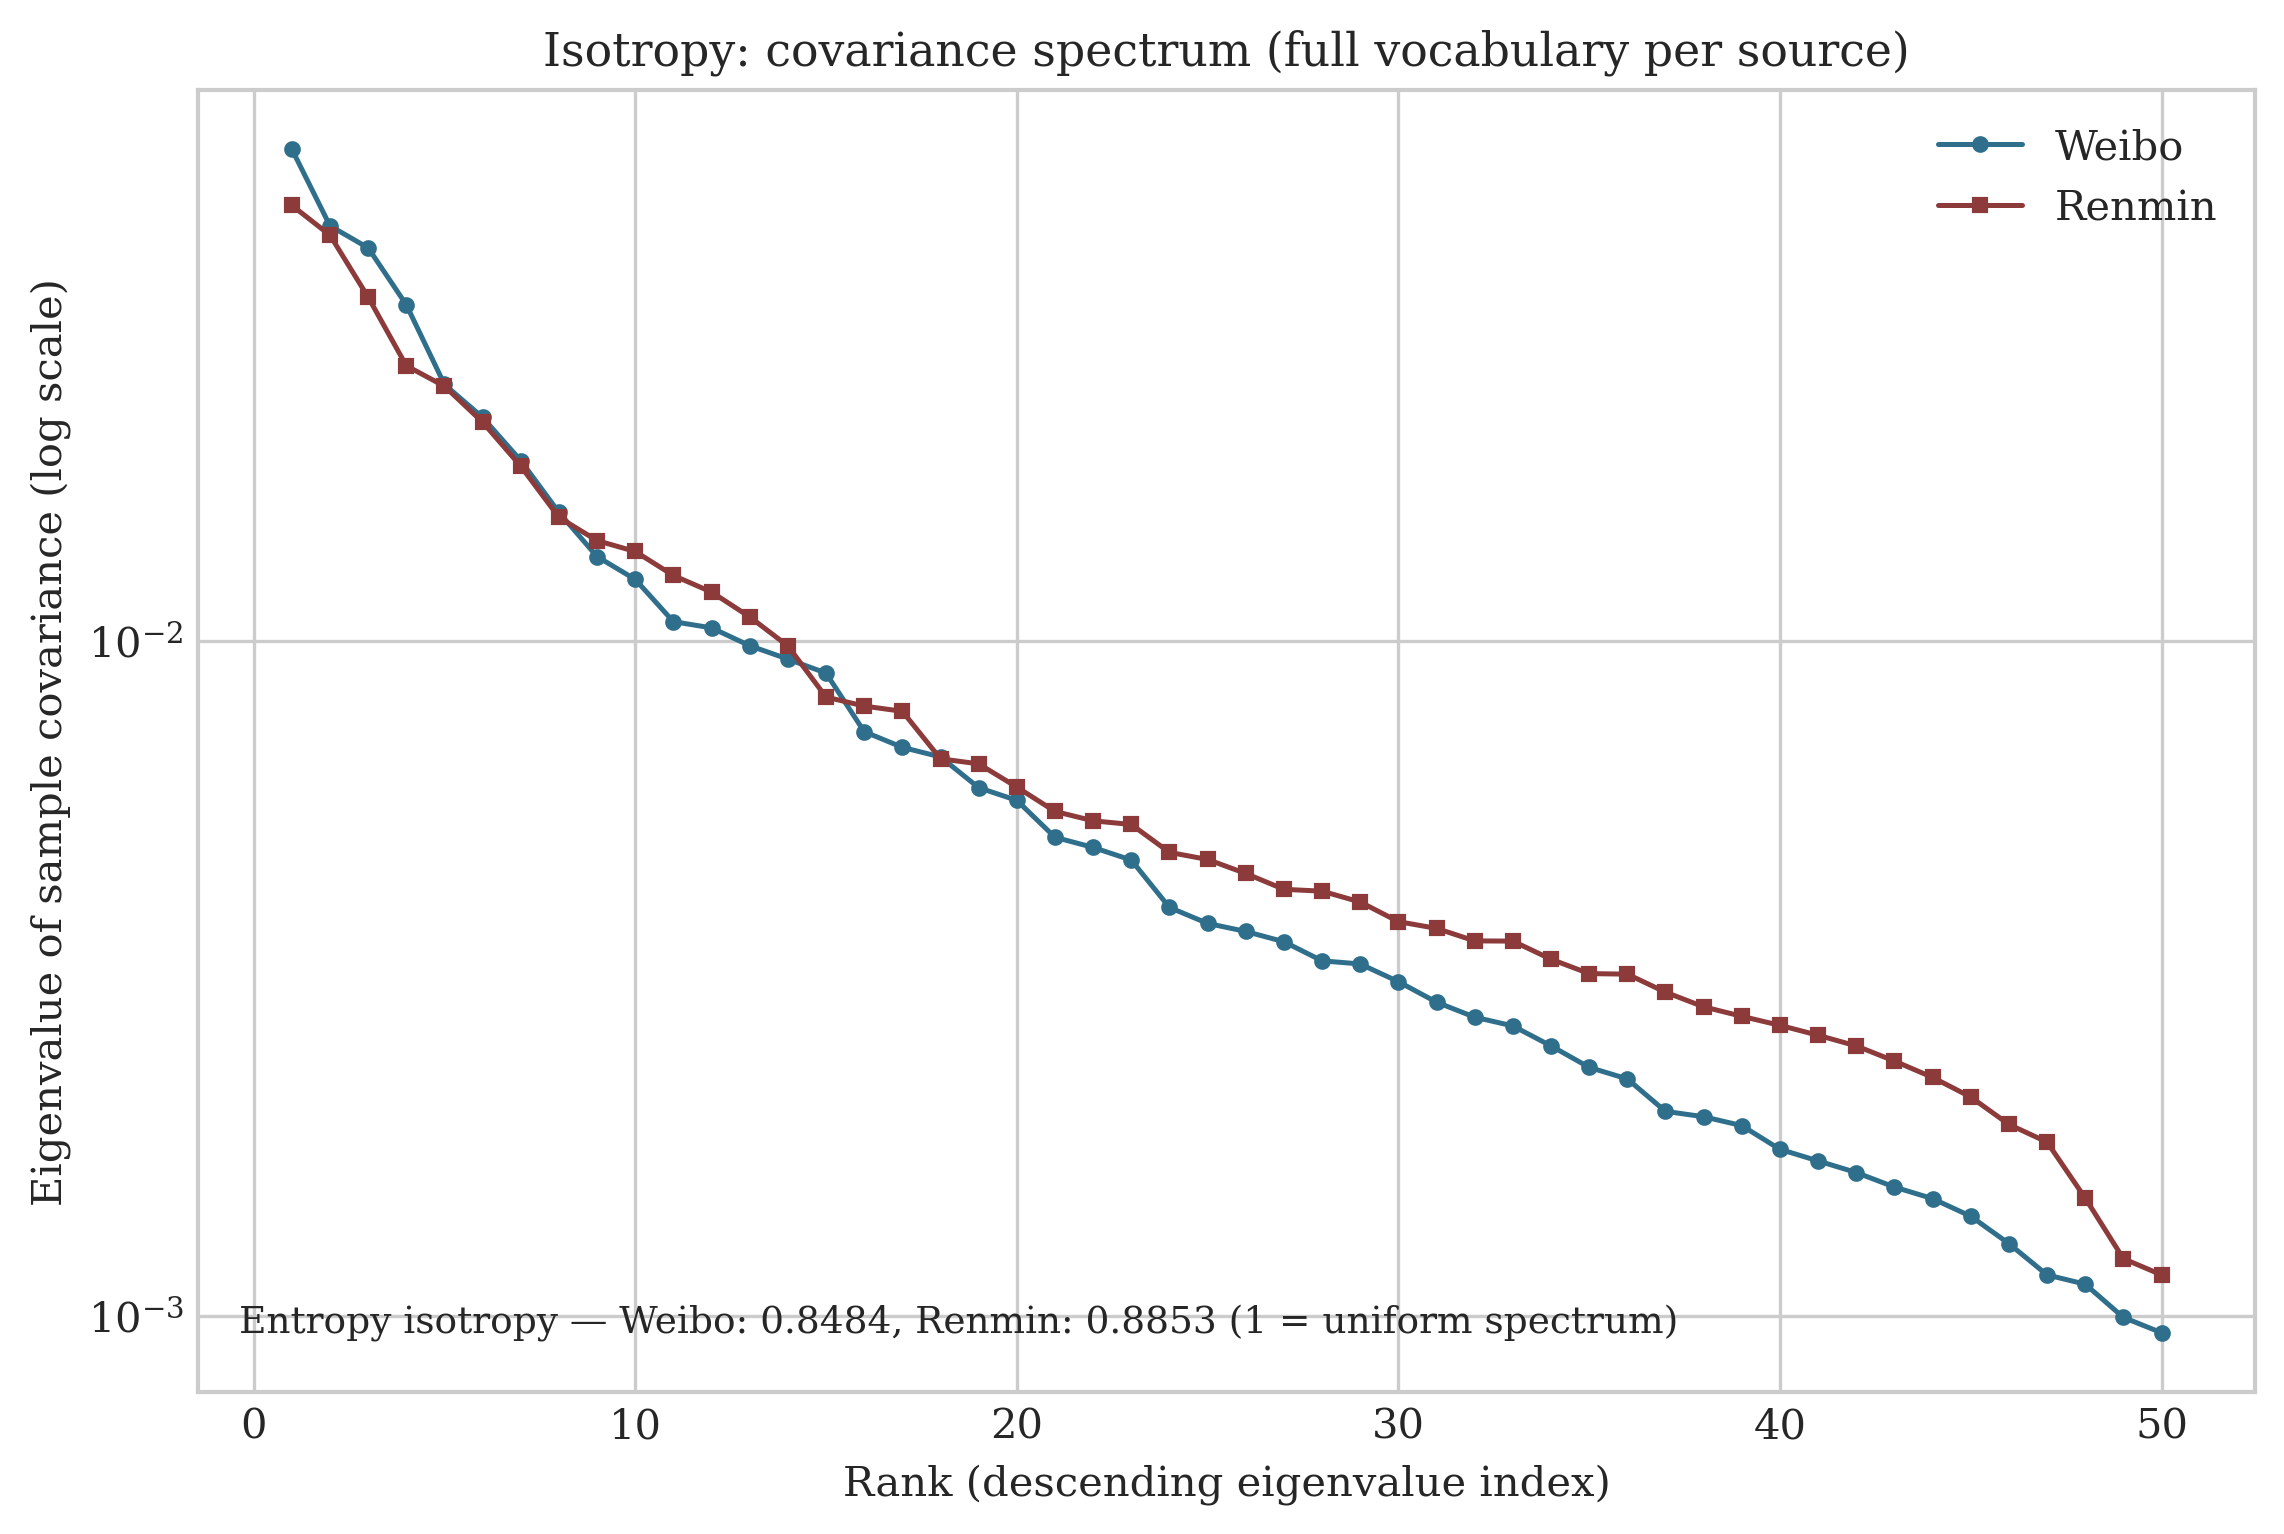
\includegraphics[width=0.7\linewidth]{geometric_space_covariance_isotropy_spectrum.png}}{%
    \fbox{\parbox[c][0.18\textheight][c]{0.88\linewidth}{\centering 协方差谱图}}}
  \caption{几何级协方差：特征值及方差份额谱。}
  \label{fig:geom-cov-spectrum}
\end{figure}

\begin{figure}[htbp]
  \centering
  \IfFileExists{./figures/geometric/geometric_space_covariance_logdet_breadth.png}{%
    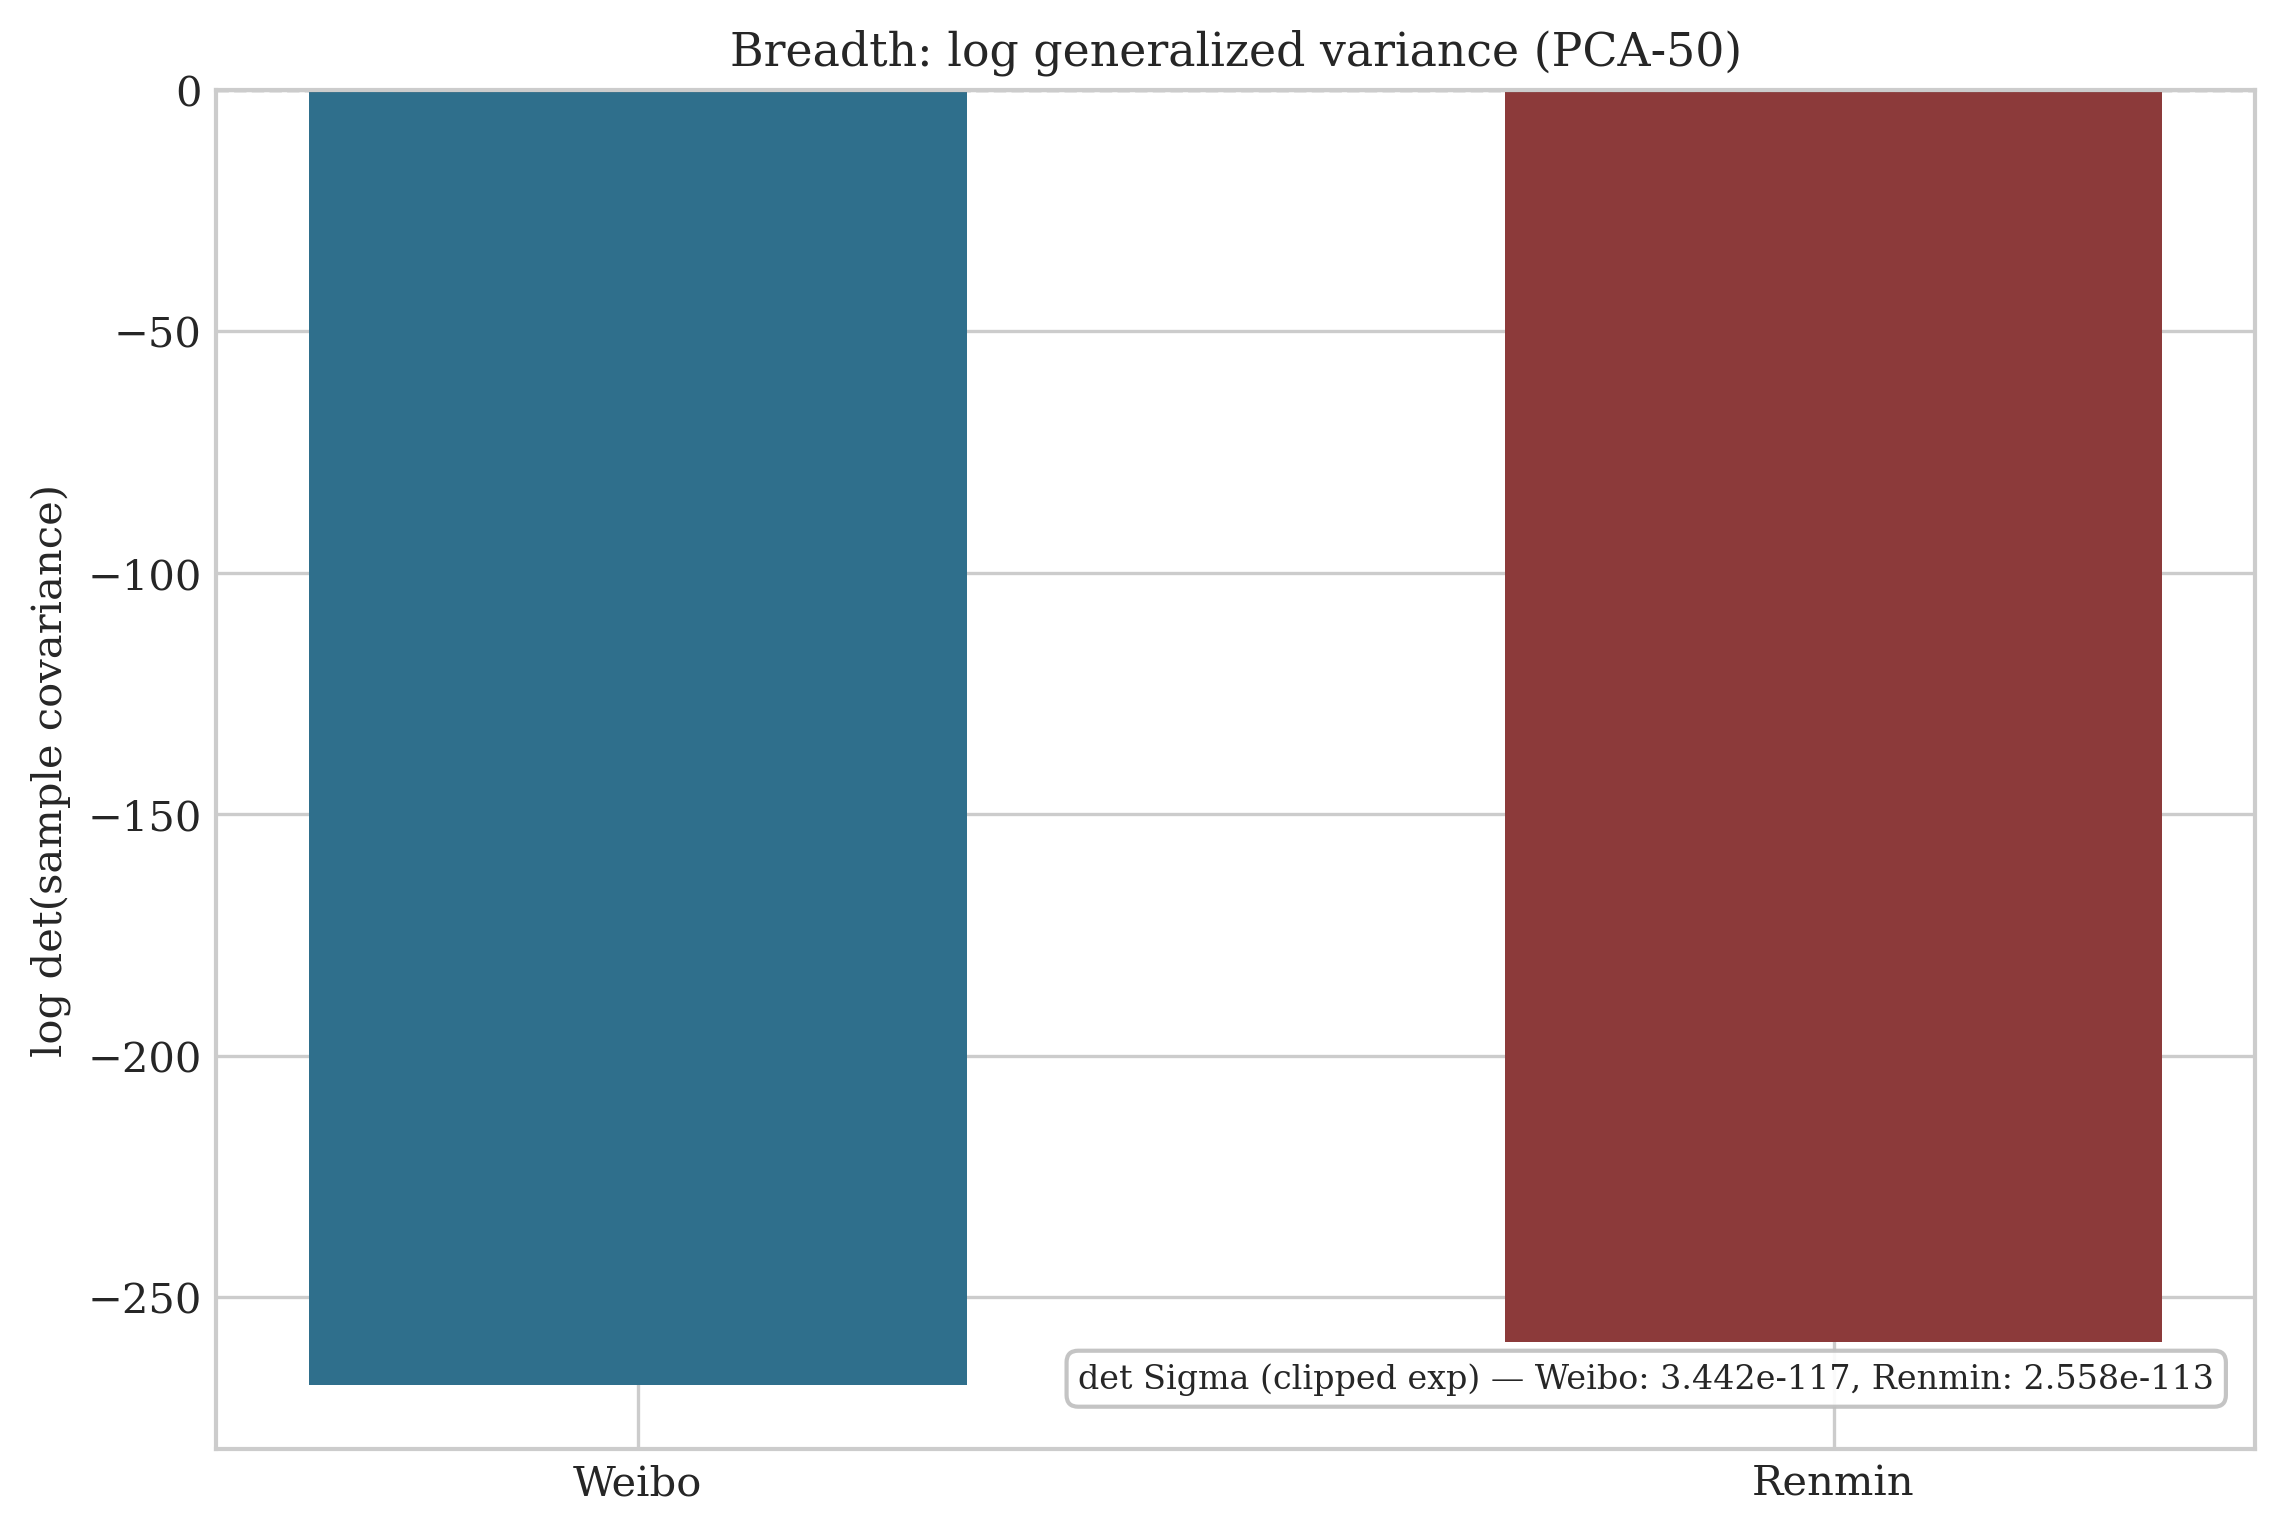
\includegraphics[width=0.7\linewidth]{geometric_space_covariance_logdet_breadth.png}}{%
    \fbox{\parbox[c][0.18\textheight][c]{0.88\linewidth}{\centering logdet 柱状图}}}
  \caption{几何级协方差：对数广义方差 $\log\det\hat{\boldsymbol{\Sigma}}$ 对比。}
  \label{fig:geom-cov-logdet}
\end{figure}

\FloatBarrier

\subsection{子空间叠合残差：交集词上的正交普鲁克}

\subsubsection{定义与公式}
设两侧词向量键集合之交为 $\mathcal{V}$，表~\ref{tab:geom-proc} 中“交集词表规模”即 $|\mathcal{V}|$。
\textbf{优化与标量指标并非在全体 $|\mathcal{V}|$ 行上计算}：实现中自 $\mathcal{V}$ 内\textbf{均匀随机无放回}
抽取至多 $n{=}12000$ 个词（固定随机种子），仅将这些词投影到联合 PCA-50 后堆成微博矩阵 $Z_{\mathrm{wb}}$ 与
人民日报矩阵 $Z_{\mathrm{rm}}$，行按同一词对齐。对两矩阵分别\textbf{列去中心化}（各自在该 $n$ 行子矩阵上
逐列减均值）后仍记为 $Z_{\mathrm{wb}},Z_{\mathrm{rm}}$，求正交矩阵
$R\in\mathbb{R}^{50\times 50}$ 使 Frobenius 残差最小：
\begin{equation}
  R^\star \in \arg\min_{R^{\mathsf{T}}R=I_{50}} \bigl\lVert Z_{\mathrm{wb}}R-Z_{\mathrm{rm}}\bigr\rVert_F^2,\qquad
  \mathbf{E}=Z_{\mathrm{rm}}-Z_{\mathrm{wb}}R^\star .
\end{equation}
\textbf{相对残差平方}定义为 
\begin{equation}
  \frac{\lVert\mathbf{E}\rVert_F^2}{\lVert Z_{\mathrm{rm}}\rVert_F^2}
\end{equation}
其中分母取人民日报侧\textbf{已去中心化}矩阵的 Frobenius 范数平方（与表~\ref{tab:geom-proc} 一致），以便与
$\lVert\mathbf{E}\rVert_F^2$ 在同一尺度下比较；二者均\textbf{仅}由上述 $n\le12000$ 行汇总。

\subsubsection{指标含义}
该步骤检验的是：在\textbf{已固定}的联合 PCA-50 基底下，交集词在两域中的坐标是否仍可通过\textbf{一次}
正交旋转相互逼近。相对残差接近 $0$ 表示子空间内仍可正交叠合；接近 $1$ 则表示即便允许旋转，两域点集
在该子空间中仍\textbf{明显不一致}。须与第三节区分：第三节的 $Q$ 作用于 $300$ 维对齐并基于锚点估计；
此处的 $R$ 作用于\textbf{同一} PCA-50 工作坐标，对象是\textbf{交集内参与优化的随机子样本}词坐标行
（至多 $12000$ 行），回答“整体拓扑是否一致”的问题，而非重复估计 $Q$，亦非在全交集上再求一次
$R^\star$。

\subsubsection{结果呈现与分析}

\begin{table}[htbp]
  \centering
  \caption{PCA-50 子空间普鲁克残差摘要}
  \label{tab:geom-proc}
  \begin{tabular}{@{}ll@{}}
    \toprule
    项目 & 数值 \\
    \midrule
    交集词表规模 & $138\,833$ \\
    子样本词数 & $12000$ \\
    Frobenius 残差平方 $\lVert\mathbf{E}\rVert_F^2$ & $3943.77$ \\
    相对残差平方（按上式分母） & $0.7697$ \\
    \bottomrule
  \end{tabular}
\end{table}

\ 

表~\ref{tab:geom-proc} 中 Frobenius 残差平方与相对残差平方均对应上述 $n{=}12000$ 子样本上的汇总；
其中相对残差平方约 $0.7697$，可直接解读为：在 PCA-50 工作空间内，单一正交映射解释后的剩余不一致仍占参考能量的约 $77\%$，
两域交集词几何仍存在\textbf{显著的非正交差异}。这与第六节在\textbf{同一} $\mathbf{Z}_{\mathrm{all}}$ 上观察到的簇结构差异相互印证。
图~\ref{fig:geom-proc} 的热图与按维平均残差曲线进一步给出差异的方向分布。

\begin{figure}[htbp]
  \centering
  \IfFileExists{./figures/geometric/geometric_space_topology_procrustes_residual_heatmap.png}{%
    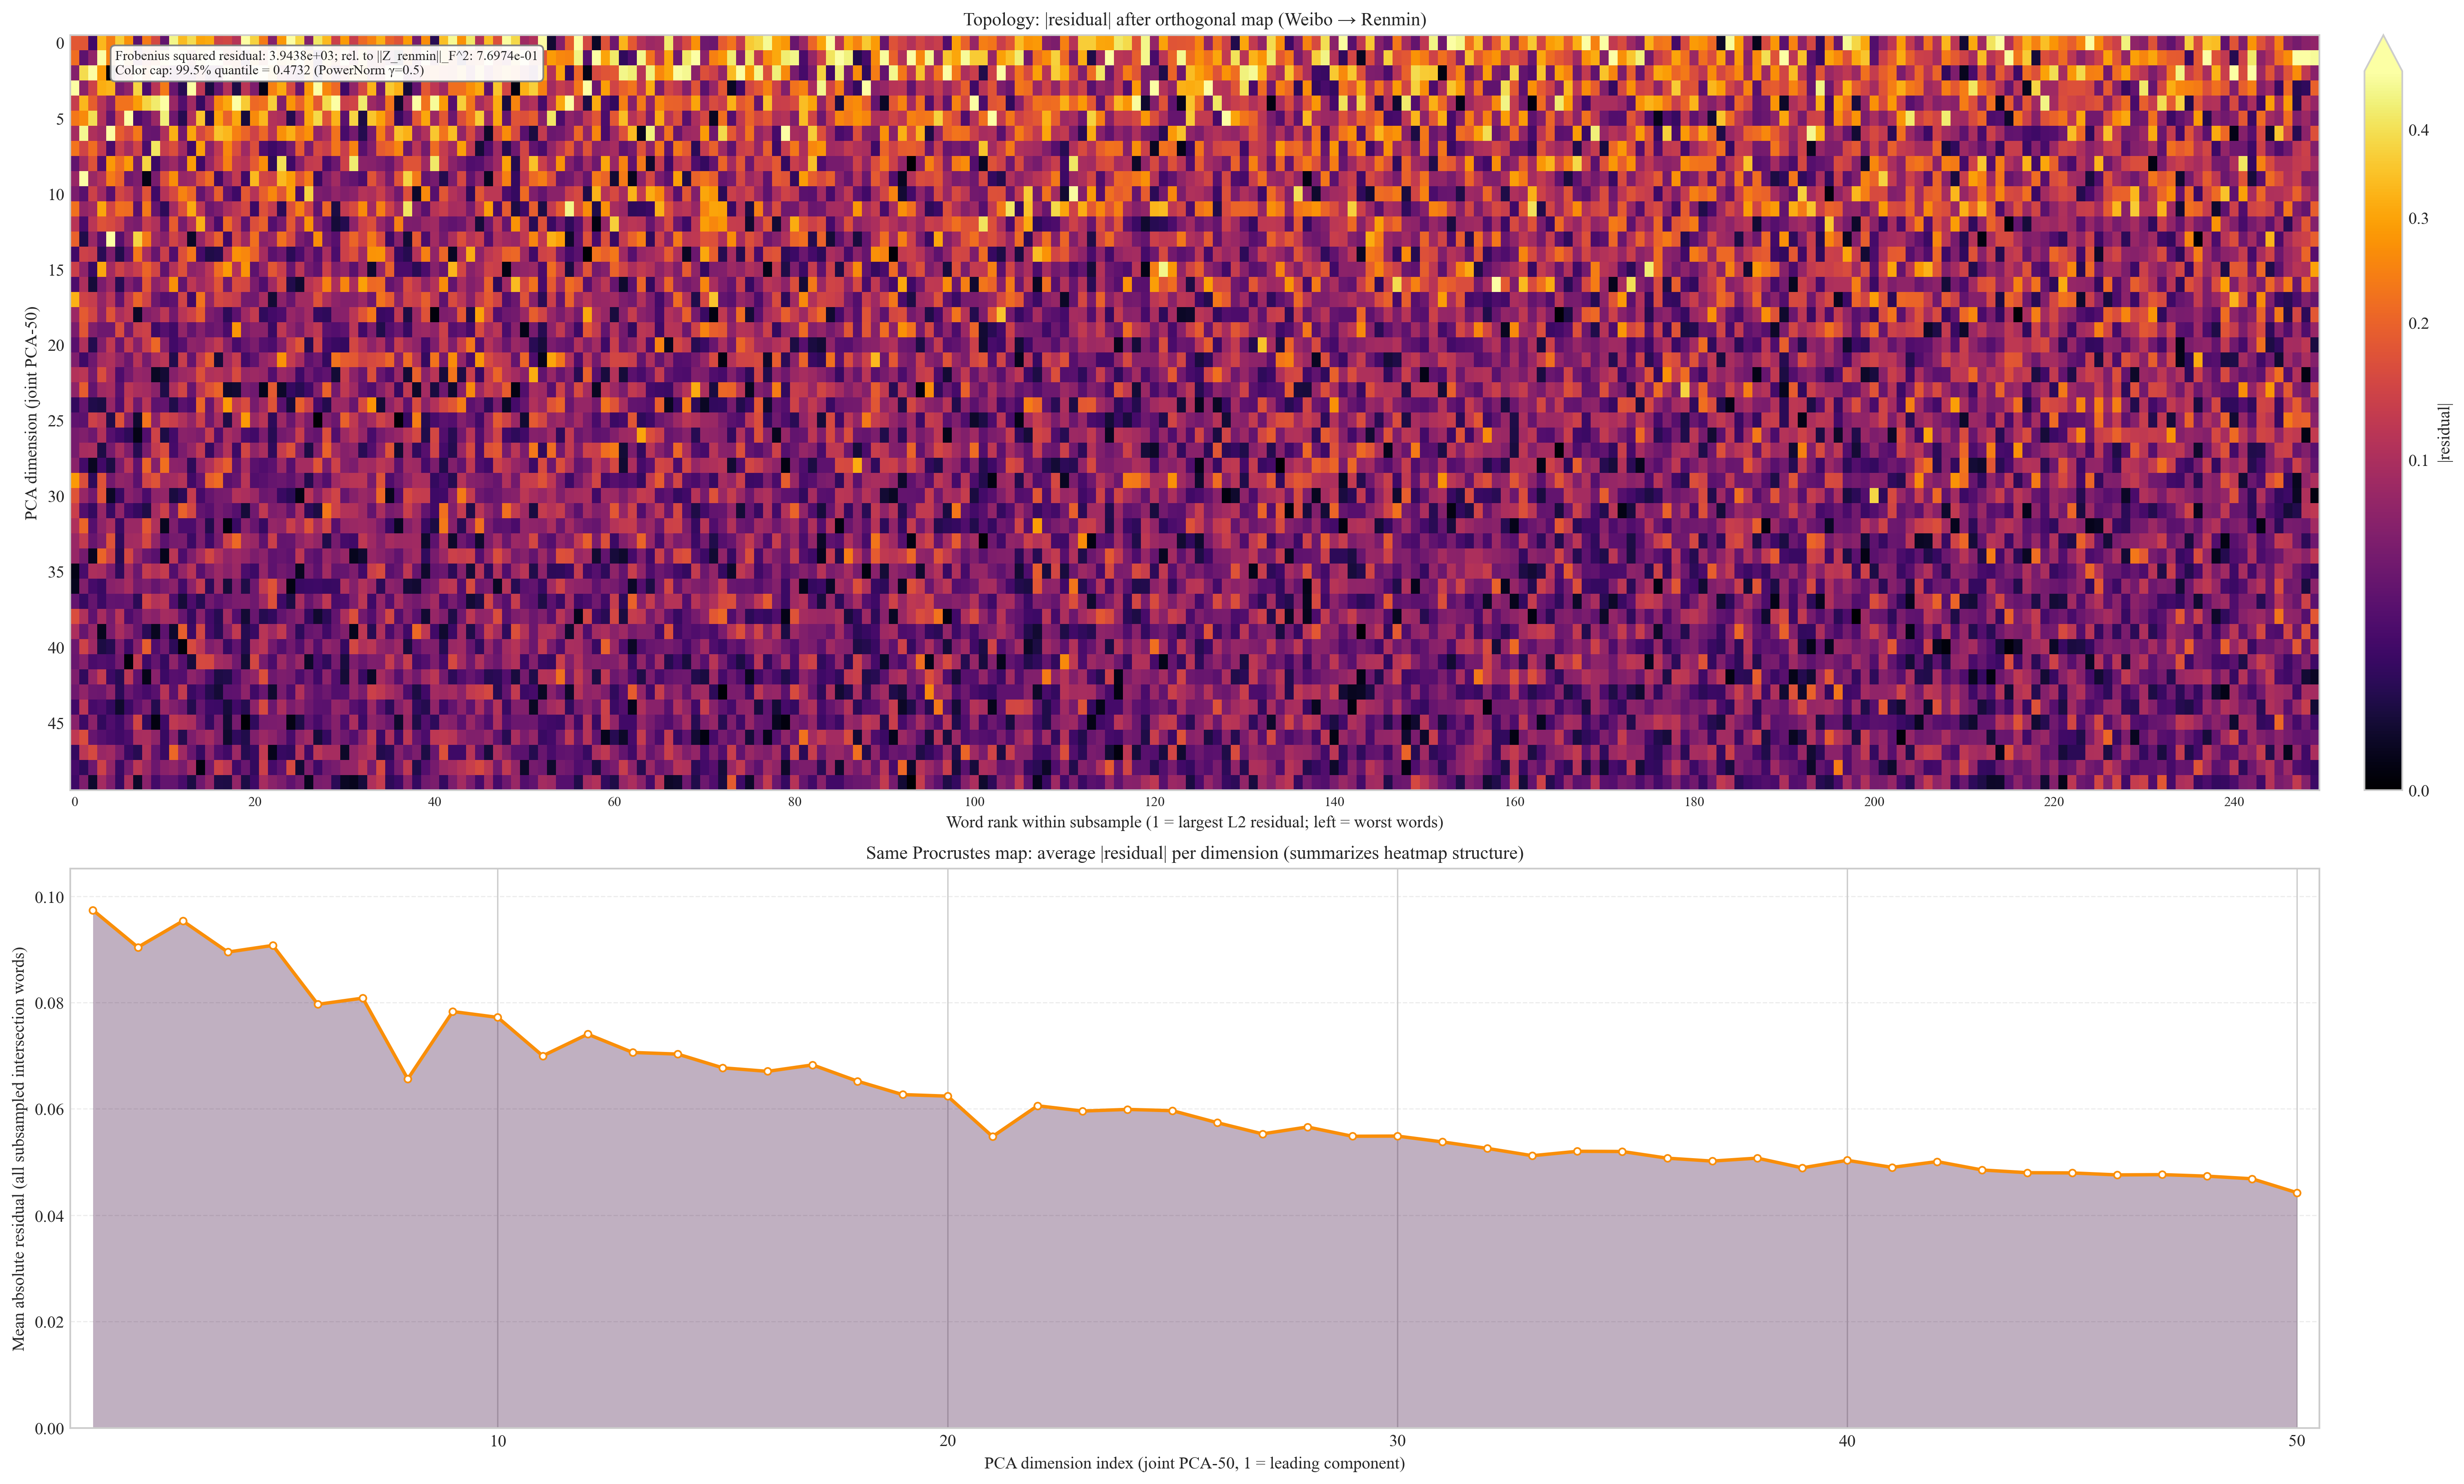
\includegraphics[width=1\textwidth]{geometric_space_topology_procrustes_residual_heatmap.png}}{%
    \fbox{\parbox[c][0.22\textheight][c]{0.90\linewidth}{\centering （插图：普鲁克残差热图与按维平均残差）}}}
  \caption{普鲁克残差: \textbf{上图}按残差欧氏范数降序取前 $250$ 词；\textbf{下图}为残差绝对值的平均。}
  \label{fig:geom-proc}
\end{figure}

\FloatBarrier
\section{评价与推广}

\subsection{评价}

\subsubsection{研究亮点}

\paragraph{多层次语义漂移指标} 词级给出 $\mathrm{Shift}(w)$ 与邻域类可排序指标；群体级在\textbf{同一}合并簇划分下比较两域质心与
可分性；几何级不依赖簇标签，补充点对距离、协方差谱与普鲁克残差。三层回答的问题不同，并列使用有利于
避免把某一种距离或某一种划分误当成漂移的全部内涵。

\paragraph{诊断样本与最终估计分离} 在群体级部分，簇数 $K$ 先在子样本上做多指标联合诊断，再回到全词表拟合一次 KMeans 并生成最终标签。
这种“诊断—估计”分离流程降低了同一样本既选参又报结论的耦合风险，使后续簇内、簇间指标的统计口径更一致、可复现性更高。

\paragraph{结果解释具备可核查路径} 词级高漂移候选先经低频专名噪声筛查，再回到语料语境做用法解释；群体级与几何级结论通过表、热图与
残差谱交叉印证。由此形成“指标发现—噪声甄别—语料复核”的闭环，提升了结论的可解释性与可审查性。

\subsubsection{误差来源与局限性}

\paragraph{表示形式与单义假设}
SGNS 为每词赋予单一向量，不区分义项；在此表示下，任何“漂移”度量本质上都是\textbf{用法分布}
在固定坐标中的投影，而非义项级精细语义。

\paragraph{高频与低频的估计方差}
罕用专名、人名地名等在两侧共现极稀疏，向量方向不稳定，$\mathrm{Shift}(w)$ 等标量易\textbf{虚高}，
与“真实语义变化”不可等同；从较大候选集合中人工剔除专名可改善展示，但无法从估计上根除低频噪声。
词级 Jaccard 与群体级簇统计在稀疏词占主导的簇上同样会放大该问题。

\paragraph{语料差异与解释边界}
本文设定为\textbf{横截面}下人民日报与微博两路静态嵌入的并列比较，在此前提下，词级与邻域上的差异应
主要联系两语料在主题、语体与话题覆盖上的系统不同，概括为
\textbf{跨语料、跨语境的用法差别}；解释结论时不宜脱离这一数据类型作过度外推。

\paragraph{降维、聚类与几何诊断}
联合 PCA-50 截断后方差分配与全维不同，几何量与普鲁克残差均在该工作子空间内陈述，宜作相对比较。
KMeans 隐含近似球形簇等假设，合并簇标签是工作划分而非唯一“真实主题”。第七节 PCA-50 普鲁克与第三节
$300$ 维 $Q$ 在维数、子样本与优化目标上均不同，数值上不应简单对立，须分设定阅读。

\subsection{推广}

其它\textbf{双域静态词向量}可沿用同一流程：换语料后重写锚点与频次规则，重跑对齐与诊断，再按需
调整 $K$、邻域大小 $k$ 等超参数。表示上可尝试非正交或小字典监督的映射、或换用 GMM/谱聚类等替代
KMeans；几何上可对普鲁克残差做置换检验、或在算力允许时增大子样本。若改用 BERT 类模型，对齐与
“漂移”应定义在子词或句级表示上，并单独设计存储与评测，不宜与本文 SGNS 管线直接混用。

\FloatBarrier
\section{总结与展望}

\subsection{全文工作总结}

\subsubsection{问题与总体框架}
本文针对人民日报与微博两路中文词向量，研究跨空间\textbf{可比性建立}与可比建立后的\textbf{语义漂移系统刻画}。
核心认识是：未经处理的欧氏坐标差异同时混杂\textbf{基选择与训练诱导的非语义自由度}与\textbf{真实域间语义差异}，
故须先在对齐假设下分离前者，再在词级、群体级与几何级上分层汇总后者。

\subsubsection{跨域对齐（第三节）}
在交集高频锚点上，以行 L2 归一化后的\textbf{正交普鲁克}迭代估计微博侧映射 $Q$，并结合 CSLS 思想
筛选锚点，使估计对伪近邻具有一定稳健性。对齐产物经 $Q^{\mathsf{T}}Q$ 等检验与分词表诊断后，可认为
在 $300$ 维上已构造出与人民日报侧\textbf{可比的微博坐标系}；同时，诊断所揭示的\textbf{非均匀改善}
表明：对齐解决的是可比性，而非消去全部语义差别。

\subsubsection{词级语义漂移（第四节）}
在映射后的统一空间中，以 $\mathrm{Shift}(w)$、邻域重叠与 Jaccard 型指标等刻画\textbf{单个词}的
方向移动与邻域重排；结合功能词阈值与专名噪声讨论，词级结果宜解释为\textbf{局部、可复核}的跨语境
差异信号，对应横截面双域比较下的用法分布差别。

\subsubsection{联合 PCA-50 工作表示（第五节）}
两域词向量经行 L2 归一化后纵向拼接，联合拟合 PCA，取前 $50$ 维得到 $\mathbf{Z}_{\mathrm{all}}$。
该矩阵专供第六节、第七节在可控维数下做聚类、协方差与几何量计算；\textbf{词级分析仍在对齐后的
约 $300$ 维邻域中进行}，二者并列，互不替代。

\subsubsection{群体级语义漂移（第六节）}
在 $\mathbf{Z}_{\mathrm{all}}$ 上，先在子样本做多指标簇数诊断并取 $K{=}20$，再对全词表拟合
KMeans 得到合并簇标签。在此\textbf{固定划分}下计算簇内跨域质心漂移、簇内紧致度，以及分域簇间距离、
轮廓系数等可分性指标。这些量依赖于“联合 PCA + 该次 KMeans”的约定，应理解为该划分下的结构化摘要。

\subsubsection{几何级形态与拓扑诊断（第七节）}
不依赖簇标签：用点对距离、各源协方差谱与 $\log\det$ 等描述整体尺度与二阶差异；在交集词的 PCA-50
子样本上做正交普鲁克，检验\textbf{同一词}两域坐标能否经单一正交变换近似重合。与第六节相比，几何级
侧重无标签的整体形态与词行对齐残差。

\subsection{研究展望}

\subsubsection{锚点与映射}
在\textbf{锚点构造与映射族}上可引入词典信息、人工种子或弱监督分类，并与 CSLS 等分数联合排序；
映射可在正交之外尝试含平移、尺度的刚性族或带正则的可逆线性族，同时以 held-out 锚点与敏感性分析
报告推广误差，避免单次估计过拟合。

\subsubsection{聚类、几何与统计推断}
在\textbf{聚类与几何指标}上可补充置换检验、自助法等以刻画随机波动；聚类算法可换用混合模型、
谱聚类或层次方法作对照。工作坐标除联合 PCA 外，可对随机投影、CCA 型跨视图子空间等做截断方式的
敏感性分析，再观察群体级与几何级结论是否稳定。

\subsubsection{表示学习范式}
若由静态词向量转向\textbf{上下文嵌入}，须在子词或句级上重定义对齐单元、邻域与“漂移”度量，
并单独设计存储与评测流程，不宜与本文 SGNS 管线直接混用。

\begin{thebibliography}{99}
% 词向量表示与数据资源（问题分析、摘要、第三节背景）
\bibitem{mikolov2013efficient}
Mikolov T., Chen K., Corrado G., Dean J.
Efficient Estimation of Word Representations in Vector Space.
arXiv:1301.3781, 2013.

\bibitem{mikolov2013distributed}
Mikolov T., Sutskever I., Chen K., Corrado G., Dean J.
Distributed Representations of Words and Phrases and their Compositionality.
In Advances in Neural Information Processing Systems, vol.~26, 2013.
arXiv:1310.4546.

\bibitem{pennington2014glove}
Pennington J., Socher R., Manning C.~D.
GloVe: Global Vectors for Word Representation.
In Proceedings of EMNLP, 2014.

\bibitem{chinese-word-vectors}
Chinese Word Vectors 开源项目（多领域、多表示中文预训练词向量资源与说明）.
Embedding/Chinese-Word-Vectors, GitHub repository:
\url{https://github.com/Embedding/Chinese-Word-Vectors}, 2018.

% 语义空间对齐（第三节）
\bibitem{schonemann1966procrustes}
Sch\"onemann P.~H.
A generalized solution of the orthogonal Procrustes problem.
\emph{Psychometrika}, 31(1):1--10, 1966.

\bibitem{artetxe2018robust}
Artetxe M., Labaka G., Agirre E.
A robust self-learning method for fully unsupervised cross-lingual mappings of word embeddings.
In Proceedings of ACL, pages 789--798, 2018.

\bibitem{conneau2018word}
Conneau A., Lample G., Ranzato M., Denoyer L., J\'egou H.
Word Translation without Parallel Data.
In Proceedings of ICLR, 2018.

% 语义漂移与历时/跨域嵌入综述、词级度量（第四节及评价）
\bibitem{kutuzov2018survey}
Kutuzov A., {\O}vrelid L., Szymanski T., Velldal E.
Diachronic Word Embeddings and Semantic Shifts: A Survey.
In Proceedings of COLING, pages 1384--1397, 2018.

\bibitem{hamilton2016diachronic}
Hamilton W.~L., Leskovec J., Jurafsky D.
Diachronic Word Embeddings Reveal Statistical Laws of Semantic Change.
In Proceedings of ACL, pages 1489--1501, 2016.

\bibitem{jatowt2021survey}
Jatowt A., Tahmasebi N., Borin L., Matswin S.
Survey of Computational Approaches to Lexical Semantic Change Detection.
\emph{Computational Linguistics}, 47(2):603--655, 2021.

% 几何结构、嵌入空间性质（第七节及概念漂移资料中的几何层）
\bibitem{radovanovic2010hubs}
Radovanovi\'c M., Nanopoulos A., Ivanovi\'c M.
Hubs in space: Popular nearest neighbors in high-dimensional spaces.
\emph{Journal of Machine Learning Research}, 11:2487--2531, 2010.

\bibitem{mu2018allbutthetop}
Mu J., Bhat S., Viswanath P.
All-but-the-Top: Simple and Effective Postprocessing for Word Representations.
In Proceedings of ICLR, 2018.
arXiv:1702.01417.

\end{thebibliography}

\end{document}
